\documentclass[10pt]{article}
\usepackage[utf8]{inputenc}
\usepackage[T1]{fontenc}
\usepackage{lmodern}
\usepackage[margin=0.75in]{geometry}
\usepackage{amsmath,amssymb,amsthm,mathtools}
\usepackage{booktabs,longtable,array,tabularx}
\usepackage{graphicx}
\usepackage{float}
\usepackage{xcolor}
\usepackage{hyperref}
\usepackage{url}
\usepackage{enumitem}
\usepackage{caption}
\usepackage{microtype}
\hypersetup{colorlinks=true,linkcolor=blue,citecolor=blue,urlcolor=blue}
\setlength{\parskip}{0.47em}
\setlength{\parindent}{0pt}
\setlist[itemize]{leftmargin=1.25em,itemsep=0.15em,topsep=0.25em}
\setlist[enumerate]{leftmargin=1.5em,itemsep=0.15em,topsep=0.25em}
\emergencystretch=3em
\sloppy
\newtheorem{definition}{Definition}
\newtheorem{lemma}{Lemma}
\newtheorem{proposition}{Proposition}
\newtheorem{empirical}{Empirical Result}
\newtheorem{protocol}{Protocol}
\newcommand{\SY}{\mathfrak{S}_Y}
\newcommand{\CHLone}{\mathrm{CHL1}}
\newcommand{\CHLtwo}{\mathrm{CHL2}}
\newcommand{\Epath}{E_Y^{\mathrm{path}}}
\newcommand{\Omegapath}{\Omega_Y^{\mathrm{path}}}
\newcommand{\loglik}{\ell}
\title{A Conditional Hardy--Littlewood Markov Kernel for Consecutive Prime Gaps}
\author{Jose Antonio Cano Gregorio}
\date{Whitepaper v1.8 --- Self-Contained Protocol and Orientation-Lifted Diagnostics}
\begin{document}
\maketitle
\begin{abstract}
We introduce CHL2, a finite conditional Markov kernel for consecutive prime gaps.  The construction starts from the Hardy--Littlewood singular series, converts the static triple-constellation weight into the conditional ratio
\[
R_Y(g_2\mid g_1)=\frac{\SY(\{0,g_1,g_1+g_2\})}{\SY(\{0,g_1\})},
\]
and then multiplies this by a first-order no-interior-prime survival factor derived from conditional four-point singular-series ratios.  Thus CHL2 is not a replacement for Hardy--Littlewood; it is a row-normalized conditional factorization designed for the consecutive transition $g_1\mapsto g_2$.

The DS1 audit covers ten chronological pair-count blocks in the interval $[10^{11},10^{11}+2\cdot10^9]$, with $78{,}934{,}825$ observed transitions and finite support $g\le2400$.  At truncation horizon $Y=47$, CHL2 improves the CHL1 ratio-only kernel in all principal strata, and the sign of the improvement is stable under the sweep $Y\in\{31,47,61,73\}$.  It also outperforms zero-memory Cramer--Granville baselines in the conditional likelihood audits.

A new correction concerns modular diagnostics.  We formalize, as a diagnostic operator for gap kernels, the valid-edge projection from gap-residue populations to reduced-residue transition matrices.  If $p_r=P(g\equiv r\pmod q)$, the mass $p_r$ must be distributed over the $N_r(q)$ valid directed edges $b\to b+r$ in the reduced-residue graph before row normalization.  The underlying edge multiplicity is already visible in Tao's exposition of the Lemke Oliver--Soundararajan bias, while Holt's gap-population framework addresses the inter-class population problem and explicitly notes intra-class distribution across ordered residue pairs as a separate open question.  The present contribution is to use this multiplicity as an explicit row-wise projection rule for model-produced gap-residue populations.  Applied to CHL2, the orientation-lifted diagnostic resolves the apparent $q=3$ anomaly of the naive direct diagnostic and substantially improves the diagnostics for $q=5,7,11,13$.  The reproducibility suite implements the full audit pipeline, including runtime telemetry, and the core DS1 audits run on ordinary multicore hardware in minutes rather than days.

\end{abstract}
\tableofcontents
\listoffigures
\newpage

\section{Introduction}
Classical Hardy--Littlewood heuristics assign weights to admissible constellations \cite{hardy-littlewood}.  For example, the triple
\[
H_3(g_1,g_2)=\{0,g_1,g_1+g_2\}
\]
can be given a singular-series weight.  That static weight is not yet a transition law for consecutive gaps.  A model for consecutive prime gaps must answer a different question: after a gap $g_1$ has just occurred, how should the next candidate gap $g_2$ be weighted?

The construction in this paper proceeds slowly and deliberately.  First, we condition the triple weight on the already-observed pair $H_2(g_1)=\{0,g_1\}$.  Second, we penalize possible primes in the interior of the future gap.  Third, we normalize row-wise to obtain a Markov kernel.  Finally, when comparing prime-residue transitions, we lift the resulting gap-residue population to an oriented matrix of reduced-residue transitions.

\begin{figure}[H]\centering
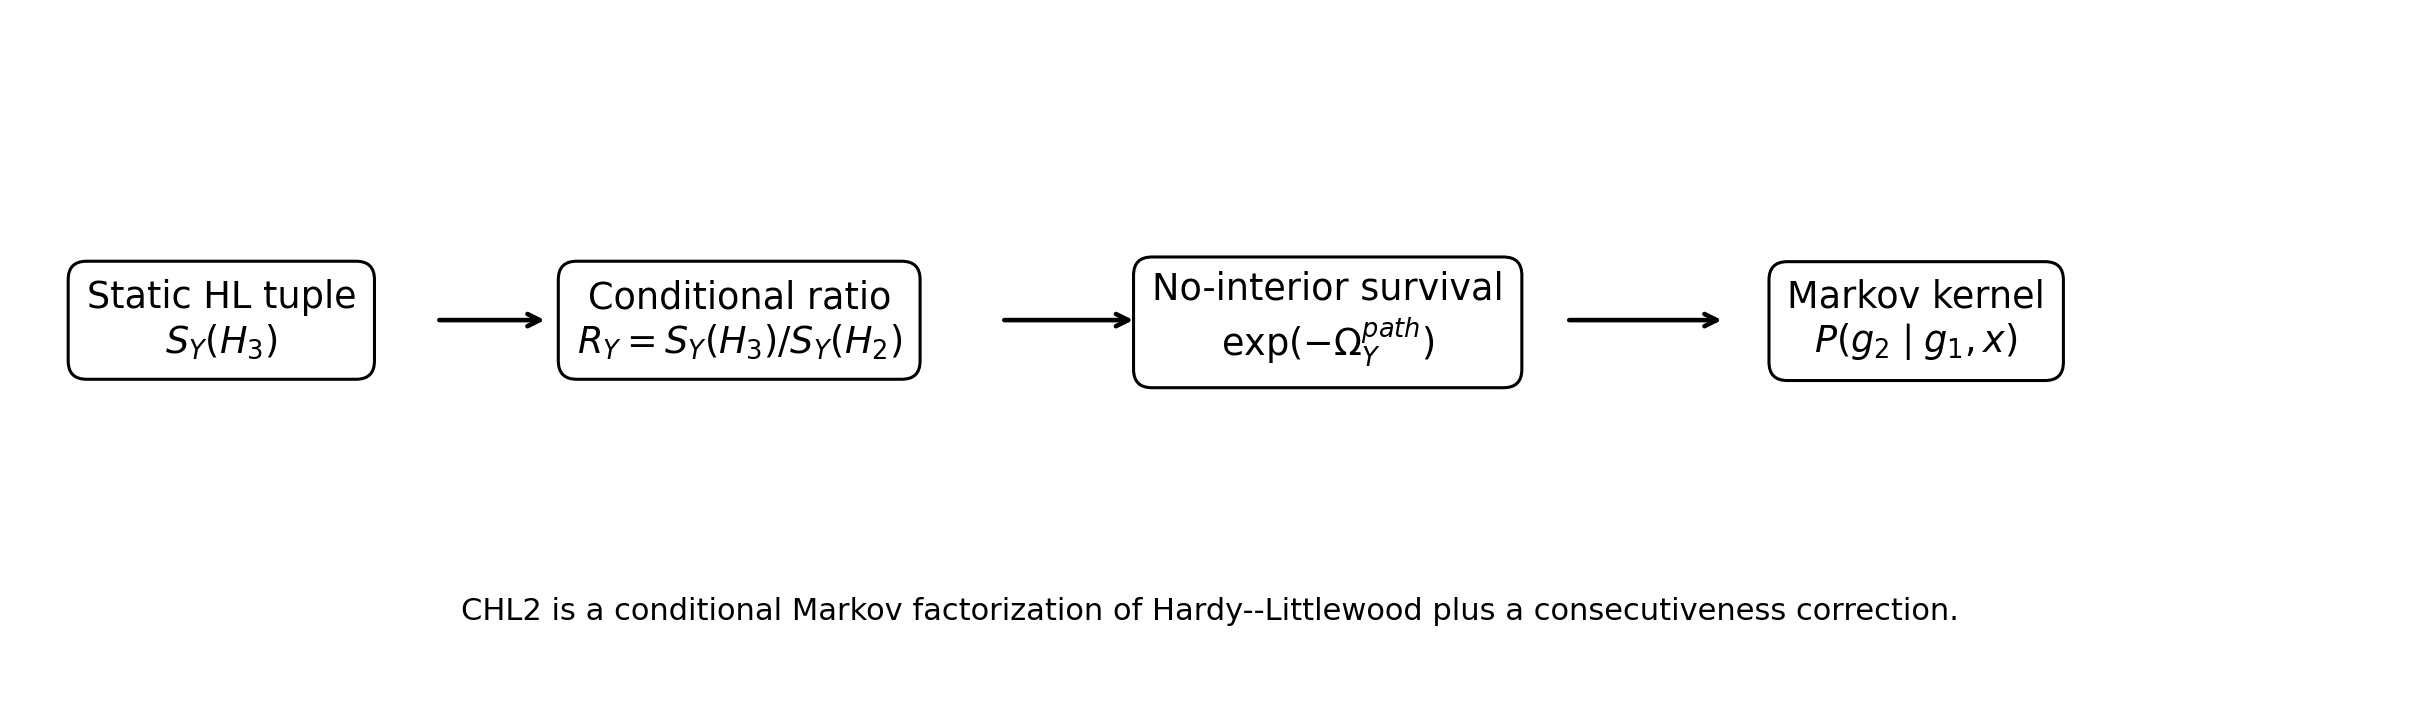
\includegraphics[width=0.96\textwidth]{figures/fig01_construction_chain.png}
\caption{Conceptual path from the static Hardy--Littlewood tuple weight to the CHL2 conditional Markov kernel.  The notation in the diagram is introduced formally in Sections~\ref{sec:chl-kernels} and~\ref{sec:orientation_lift}.}\label{fig:construction_chain}
\end{figure}

Figure~\ref{fig:construction_chain} is the intended reading guide for the paper.  Each arrow in the diagram corresponds to a mathematical obstruction that has to be removed: static tuple weights are not conditional probabilities; endpoint constellations are not necessarily consecutive gaps; gap-residue populations are not yet row-wise prime-residue transitions.  The sections below follow those obstructions in order.

This article is deliberately conservative.  It does not propose a new singular series.  It does not replace sieve theory.  It asks whether a conditional singular-series kernel, corrected for no-interior survival, predicts observed consecutive-gap transitions better than natural order-zero baselines.

\subsection{Main contributions}
The main contributions are as follows.
\begin{enumerate}
\item A conditional kernel CHL1 obtained from the singular-series ratio $\SY(H_3)/\SY(H_2)$.
\item A consecutive-gap kernel CHL2 obtained by multiplying CHL1 by a first-order no-interior survival factor.
\item A DS1 likelihood audit showing that CHL2 improves CHL1 and zero-memory baselines.
\item A cutoff sweep showing that the sign of the CHL2-vs-CHL1 gain is stable for $Y\in\{31,47,61,73\}$ in all principal strata.
\item An orientation-lifted modular diagnostic: Holt's gap-population framework addresses the inter-class distribution of gap residues, while leaving intra-class distribution across ordered residue pairs as a separate question.  We formalize the valid-edge projection from gap-residue populations to reduced-residue transition matrices, providing a model-agnostic diagnostic for this intra-class assignment.  Applied to CHL2, the projection resolves the apparent $q=3$ failure of the naive direct diagnostic and improves diagnostics for $q=5,7,11,13$.
\item Negative-control documentation explaining why empirical geometry, second-order low-wheel cumulants, and a local Lemke Oliver--Soundararajan (LOS) projection are not used as the final core model.
\end{enumerate}


\section{Related work}
\subsection{Consecutive-prime residue biases}
The modular part of this paper sits in the line of work initiated by Lemke Oliver and Soundararajan, who showed that consecutive prime pairs are not uniformly distributed among reduced-residue pairs modulo $q$ and explained the observed biases using Hardy--Littlewood heuristics \cite{lemke-sound}.  We write LOS for Lemke Oliver--Soundararajan.  When the paper later refers to an OS diagnostic, it means an Oliver--Soundararajan-style diagnostic of the transition matrix of consecutive prime residues, not a separate probabilistic model.  Tao's exposition gives a particularly transparent account of the $q=3$ case and of the combinatorial multiplicity that favors some gap residues over others \cite{tao2016biases}.  In that direct counting direction, a gap divisible by $3$ has two possible reduced starting classes, whereas a nonzero gap residue has only one.

\subsection{Gap populations and inter-class bias}
Holt's work is especially close to the present diagnostic viewpoint.  His gap-population framework studies how populations of small gaps evolve through stages of the Eratosthenes sieve and how those populations are assigned to residue classes \cite{holt2016,holt2024}.  In this language, a \emph{gap population} is the aggregate mass carried by a residue class of gaps, such as all gaps satisfying $g\equiv r\pmod q$.  Holt's population model asks an \emph{inter-class} question: how much mass belongs to each gap-residue class as the sieve evolves?  This is different from the \emph{intra-class} question: once a fixed gap-residue class has some total mass, how is that mass distributed among the ordered reduced-residue pairs $(b,a)$ that realize the same class?  Holt explicitly distinguishes these two levels in his concluding discussion and does not model possible uneven intra-class distributions \cite{holt2024}.  The distinction is useful here because a gap kernel naturally produces a population
\[
p_r=P(g\equiv r\pmod q),
\]
whereas the modular diagnostic requires a row-wise transition matrix $T_q(b,a)$.  The orientation lift below supplies the null intra-class assignment associated with such a model-produced population.

\subsection{The present diagnostic}
The orientation lift used below supplies the null intra-class assignment associated with a gap-residue population.  It distributes $p_r$ over the valid directed reduced-residue edges $b\to b+r$ and then normalizes by row.  The contribution here is not the residue multiplicity itself, but its formalization as a model-agnostic diagnostic operator for gap kernels.  Applied to CHL2, this operator shows that the apparent $q=3$ anomaly of the naive direct diagnostic was caused by an incomplete projection from inter-class gap populations to intra-class transition rows, not by a failure of the CHL2 gap-survival kernel.  Residual deviations after this lift would define genuine intra-class bias beyond the null assignment tested here.

\subsection{Residue patterns and sieve-theoretic context}
Wu studies nonuniform patterns of consecutive prime residues modulo prime moduli and connects such patterns to Hardy--Littlewood $k$-tuple heuristics \cite{wu2019}.  Lau studies existence and lower bounds for residue-class patterns of consecutive primes using modifications of Maynard--Tao sieve methods \cite{lau2024}.  These works provide context for residue patterns of consecutive primes, but they do not formulate the diagnostic projection from a model-produced gap-residue population to a transition matrix used here.  The present paper remains finite and computational: it defines a conditional gap kernel, audits it on DS1, and then evaluates its modular predictions through the valid-edge lift.

\section{Preliminaries}
Let $p_1<p_2<\cdots$ be the increasing sequence of primes and let
\[
g_n=p_{n+1}-p_n.
\]
For two consecutive gaps we write
\[
g_1=p_{n+1}-p_n,\qquad g_2=p_{n+2}-p_{n+1}.
\]

\begin{definition}[Truncated singular series]
Fix a truncation horizon $Y$.  For a finite set $H\subset\mathbb Z$, define
\[
\SY(H)=\prod_{p\le Y}\frac{1-\nu_p(H)/p}{(1-1/p)^{|H|}},
\]
where $\nu_p(H)$ is the number of distinct residue classes occupied by $H$ modulo $p$.
\end{definition}

\begin{definition}[Admissibility at horizon $Y$]
A set $H$ is admissible at horizon $Y$ if
\[
\nu_p(H)<p\qquad\text{for every prime }p\le Y.
\]
If $\nu_p(H)=p$ for some $p\le Y$, the local factor vanishes and the model assigns a hard zero.
\end{definition}

All sums over future candidate gaps are over even $g_2\ge2$, since all prime gaps after $2$ are even.  The horizon $Y$ is a finite audit horizon, not an asymptotic sieve level.

\begin{lemma}[Hard-zero support]
If $H$ occupies every residue class modulo some prime $p\le Y$, then $\SY(H)=0$.  Consequently every kernel below gives zero mass to that candidate configuration.
\end{lemma}
\noindent In the likelihood audit, observed prime-gap pairs do not create $-\infty$ log-scores from this hard-zero rule.  If an observed endpoint tuple came with a saturated local obstruction, then those endpoints could not all be prime in the first place.  Hard zeros therefore remove inadmissible candidate gaps from the model support; they do not assign zero probability to observed admissible transitions.

\section{From constellations to a Markov kernel}\label{sec:chl-kernels}
\subsection{CHL1: conditional singular-series ratio}
Let
\[
H_2(g_1)=\{0,g_1\},\qquad H_3(g_1,g_2)=\{0,g_1,g_1+g_2\}.
\]
A Hardy--Littlewood singular series is a topological weight.  It tells us how local congruence obstructions favor or suppress a finite constellation, but it does not by itself know at which height $x$ the primes are being sampled.  The first step toward a transition kernel is therefore to ask a conditional question: once the first endpoint pair $H_2(g_1)$ is present, what additional singular-series cost is incurred by appending the third point $g_1+g_2$?

This gives the conditional ratio
\[
R_Y(g_2\mid g_1)=\frac{\SY(H_3(g_1,g_2))}{\SY(H_2(g_1))}.
\]
This ratio is the first source of Markov memory: the previous gap $g_1$ changes the residue pattern of the triple and therefore changes the local factors of the next candidate gap.  At this stage, however, $R_Y$ still only supplies relative arithmetic weights.  If we row-normalized these weights without a scale constraint, the resulting mean gap would be determined by the finite support and the truncation horizon rather than by the local prime density.

The prime number theorem supplies the missing scale.  Near height $x$, the unfiltered mean prime gap is approximately $\log x$.  Conceptually, the Lagrange multiplier $\eta_Y(x)$ is the maximum-entropy scale correction that would enforce the local row mean
\[
\sum_{\substack{g_2\ge2\\g_2\ \mathrm{even}}}g_2 P_Y(g_2\mid g_1;x)\approx \log x.
\]
In the finite audits, however, the support is often filtered.  On a tail-restricted stratum such as $S_{>120}$ (defined in Section~\ref{sec:strata}), the conditional support no longer represents the unconditional prime-number-theorem scale.  The operational rule used in Section~\ref{sec:protocol} is therefore: solve a single $\eta$ per model, block, and stratum so that the model mean, averaged over the empirical distribution of previous gaps $g_1$, matches the empirical mean of $g_2$ in that same block and stratum.  This rule is applied identically to every model and baseline in the same audit cell, so the scale anchor contributes no relative advantage to CHL2.

Thus the exponential factor $e^{\eta_Y(x)g_2}$ is not a fitted residual force; it is the common finite-support scale correction that converts a dimensionless topological weight into a locally scaled probability distribution.  The indicator $\mathbf 1_{\mathrm{adm},Y}^{(3)}(g_1,g_2)$ below means that the triple $H_3(g_1,g_2)$ is admissible at horizon $Y$.  With this scale anchor in place, we can define the first conditional kernel.

\begin{definition}[CHL1 kernel]
The CHL1 ratio-only kernel is
\[
P_Y^{\CHLone}(g_2\mid g_1;x)=\frac{\mathbf 1_{\mathrm{adm},Y}^{(3)}(g_1,g_2)R_Y(g_2\mid g_1)e^{\eta_Y(x)g_2}}{Z_Y^{\CHLone}(g_1;x)},
\]
with
\[
Z_Y^{\CHLone}(g_1;x)=\sum_{\substack{h\ge2\\h\ \mathrm{even}}}\mathbf 1_{\mathrm{adm},Y}^{(3)}(g_1,h)R_Y(h\mid g_1)e^{\eta_Y(x)h}.
\]
\end{definition}
On the finite even support, the log-partition is convex in $\eta_Y$ and the mean is monotone, so the anchoring equation has a unique numerical solution whenever the support has nonzero variance.  This is why $\eta_Y$ is stable numerically and why it should be interpreted as a scale anchor rather than as an empirical tuning parameter.  Appendix~\ref{app:maxent-poisson} records the short maximum-entropy derivation.

\subsection{Why CHL1 is not yet a consecutive-gap model}
CHL1 weights the endpoints $0,g_1,g_1+g_2$.  It does not exclude additional primes between $g_1$ and $g_1+g_2$.  For a true consecutive gap, every interior position $g_1+u$ must fail to be prime.

\begin{figure}[H]\centering
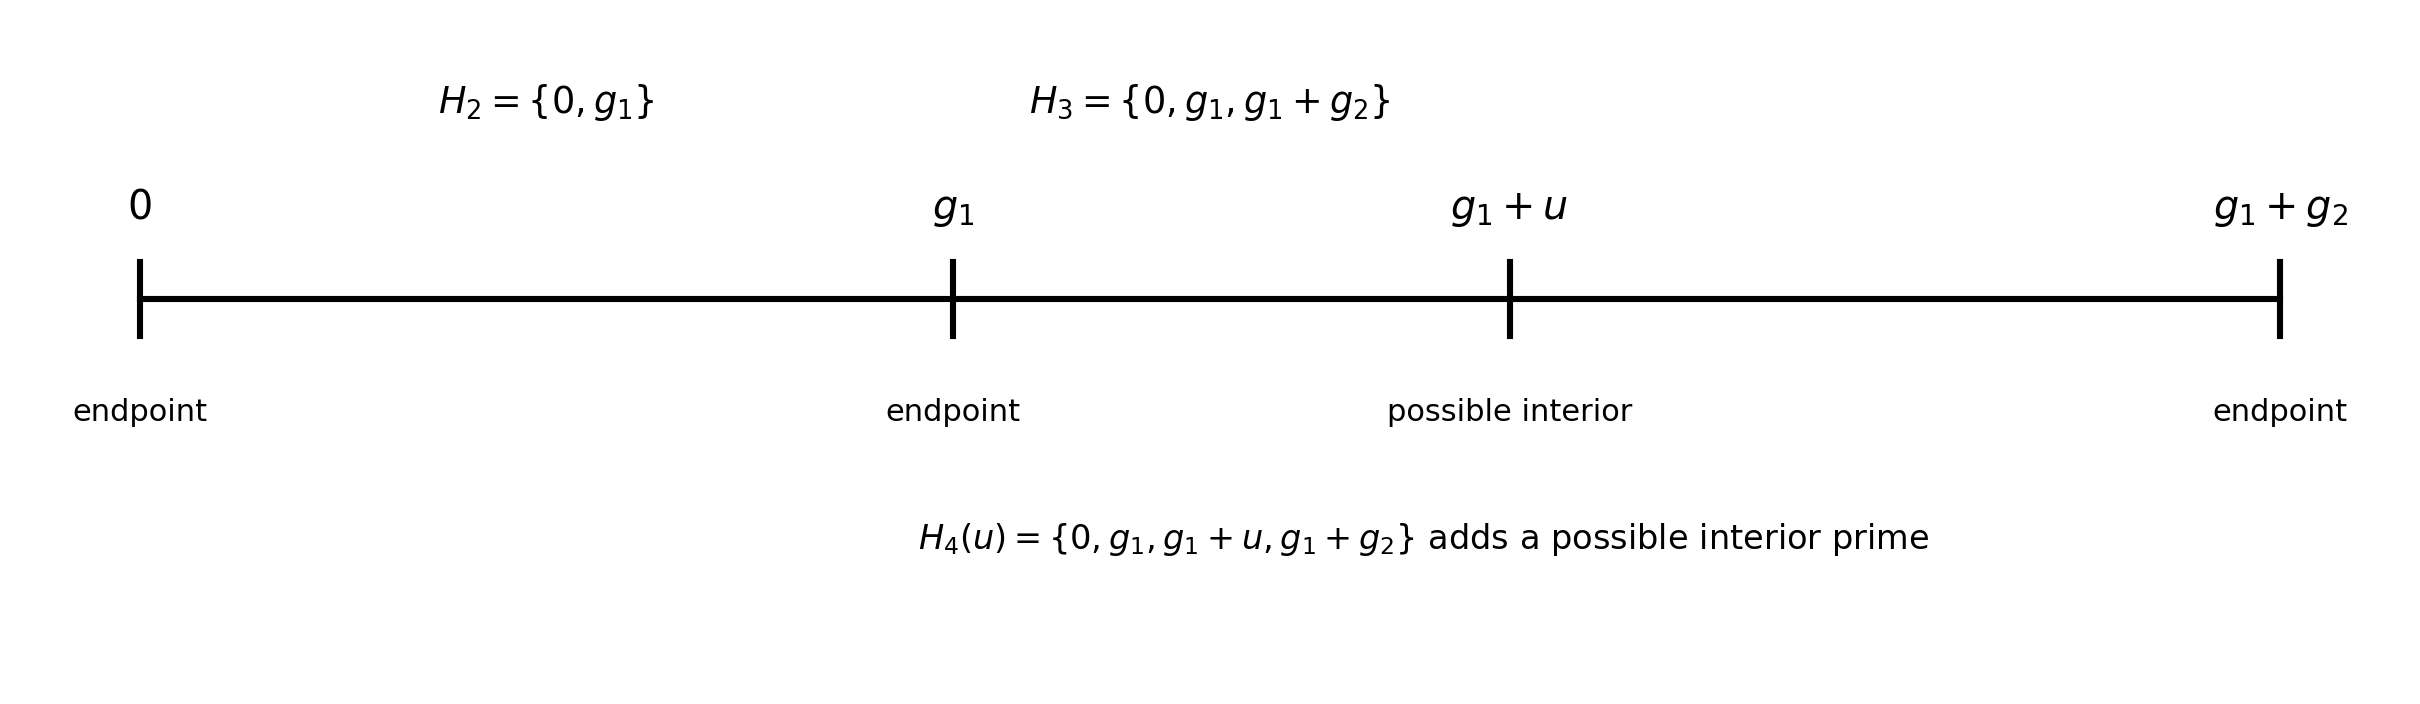
\includegraphics[width=0.96\textwidth]{figures/fig02_tuple_anatomy.png}
\caption{The endpoint constellation and the possible interior prime positions.  CHL2 is obtained by penalizing the conditional intensity of the interior positions.}\label{fig:tuple_anatomy}
\end{figure}

For each even $u$ with $2\le u\le g_2-2$, define
\[
H_4(u;g_1,g_2)=\{0,g_1,g_1+u,g_1+g_2\}.
\]
The raw probability scale for a single candidate integer near height $x$ to be prime is the prime-number-theorem density $1/\log x$.  The singular series then modulates this base density by the conditional cost of adding the interior point $g_1+u$ to the already weighted endpoint triple $H_3$.  In other words, the factor $1/\log x$ supplies the global density scale, while the ratio $\SY(H_4)/\SY(H_3)$ supplies the local arithmetic correction.

Conditioned on $H_3$, the first-order Hardy--Littlewood intensity for the interior point is therefore approximated by
\[
I_Y(u\mid g_1,g_2;x)=\frac{1}{\log x}\frac{\SY(H_4(u;g_1,g_2))}{\SY(H_3(g_1,g_2))}.
\]
Figure~\ref{fig:tuple_anatomy} shows the geometry of this term: CHL1 weights the endpoints, while CHL2 asks how many plausible interior primes those endpoints leave behind.  The first-order approximation treats the possible interior prime events as weakly dependent rare events.  If their total conditional intensity is $\Omega$, the corresponding zero-event probability is approximated by the Poisson survival probability $\exp(-\Omega)$.  Summing these intensities gives
\[
\Omegapath(g_1,g_2;x)=\sum_{\substack{2\le u\le g_2-2\\u\ \mathrm{even}}}\frac{1}{\log x}\frac{\SY(\{0,g_1,g_1+u,g_1+g_2\})}{\SY(\{0,g_1,g_1+g_2\})},
\]
and the no-interior survival factor is
\[
\Epath(g_1,g_2;x)=\exp[-\Omegapath(g_1,g_2;x)].
\]

\subsection{CHL2 kernel}
\begin{definition}[CHL2 path-exclusion kernel]
\[
P_Y^{\CHLtwo}(g_2\mid g_1;x)=\frac{\mathbf 1_{\mathrm{adm},Y}^{(3)}(g_1,g_2)R_Y(g_2\mid g_1)\Epath(g_1,g_2;x)e^{\eta_Y(x)g_2}}{Z_Y^{\CHLtwo}(g_1;x)},
\]
where
\[
Z_Y^{\CHLtwo}(g_1;x)=\sum_{\substack{h\ge2\\h\ \mathrm{even}}}\mathbf 1_{\mathrm{adm},Y}^{(3)}(g_1,h)R_Y(h\mid g_1)\Epath(g_1,h;x)e^{\eta_Y(x)h}.
\]
\end{definition}

\begin{figure}[H]\centering
\fbox{\begin{minipage}{0.92\textwidth}
\[
P_Y^{\CHLtwo}\propto
\underbrace{\mathbf 1_{\mathrm{adm}}^{(3)}}_{\text{hard support}}
\cdot
\underbrace{R_Y(g_2\mid g_1)}_{\text{conditional HL}}
\cdot
\underbrace{e^{-\Omega_Y^{\mathrm{path}}}}_{\text{no-interior survival}}
\cdot
\underbrace{e^{\eta_Y g_2}}_{\text{scale anchor}}.
\]
\end{minipage}}
\caption{Multiplicative anatomy of the CHL2 kernel.}\label{fig:kernel_anatomy}
\end{figure}


\section{Experimental protocol}\label{sec:protocol}
The formulas above define finite kernels.  The audit protocol specifies the finite support, the empirical window, the strata, the baselines, and the scoring rule.  This section is intentionally operational: it is meant to let a reader reconstruct exactly what the tables measure.


\subsection{The DS1 dataset}
DS1 is the finite prime-gap window used throughout this paper.  It consists of all observed consecutive-gap transitions in the interval
\[
[10^{11},\,10^{11}+2\cdot 10^9],
\]
with maximum recorded gap support $g_{\max}=2400$.  This cutoff is part of the finite audit design: at the DS1 scale it is roughly $95\log x$, far beyond the mass of the observed conditional distribution, while keeping every partition function finite and reproducible.  The chronological prime sequence is aggregated into pair-count tables of consecutive gaps $(g_1,g_2)$, with a count $H(g_1,g_2)$ recording how many times each pair occurs in a block.  The release audit contains ten chronological blocks, denoted B01--B10, and a total of $78{,}934{,}825$ observed transitions.

The number ten is not a mathematical parameter of the kernel.  It is an audit design choice: the blocks are large enough to give stable conditional statistics while still allowing block-level checks of sign, gain, and runtime.  The likelihood audits use the aggregated pair-count blocks.  The modular diagnostics require the same data before aggregation: the chronological prime stream.  For each consecutive pair $(p_{n-1},p_n)$ in that stream, the modular audit records the reduced-residue transition $(p_{n-1}\bmod q,p_n\bmod q)$ for each audited modulus $q\in\{3,5,7,11,13\}$.  Thus the pair-count tables are sufficient for likelihood scoring, while the empirical matrices $T_q^{\rm emp}$ are computed from chronological prime transitions.

The complete data-generation pipeline and the mapping between these mathematical objects and their computational artifacts are documented in the reproducibility section.  The local scale is held fixed at the DS1 height.  Numerically, the audits use
\[
\log x=25.328436\ldots,
\]
corresponding to the left endpoint $x=10^{11}$.  Across a two-billion interval near $10^{11}$, the relative variation in $\log x$ is below two percent.  An event-wise or block-wise $\log(p_n)$ refinement is a natural future audit, but is not used in the reported DS1 tables.

\subsection{Finite support and the multiplier \(\eta_Y(x)\)}
For each model, block, and stratum, the kernel is evaluated on the finite pair table available in that stratum.  The support is therefore the set of even candidate gaps $g_2$ appearing in the pair-count table after the stratum filter has been applied, with hard-zero admissibility factors still enforced.  Conditional models are normalized row-wise over candidates with the same previous gap $g_1$.

The multiplier $\eta_Y(x)$ is solved once per model, block, and stratum so that the model mean, averaged over the empirical distribution of previous gaps $g_1$, matches the empirical mean of $g_2$ in that same block and stratum.  It is not solved separately for every row $g_1$, it is not chosen to maximize likelihood, and it is not a fitted residual parameter.  It is the finite-support scale anchor imposed after the arithmetic weights have been specified.  On the full DS1 support this operational mean is close to the local PNT scale; on filtered strata it is the only meaningful anchor because the filter deliberately changes the mean gap.  Every baseline in the same block and stratum receives the same anchoring rule.  Equivalently, each model receives one scalar scale degree of freedom in each audit cell.  The likelihood comparisons therefore test the arithmetic shape of the weights after the common mean-gap constraint has been imposed; the anchor is not a hidden advantage available only to CHL2.


\subsection{Evaluation strata}\label{sec:strata}
The strata are deterministic filters on the observed pair $(g_1,g_2)$.  Let
\[
G_{\max}(g_1,g_2)=\max(g_1,g_2).
\]
The main text uses mathematical stratum labels rather than repository aliases:
\begin{center}\scriptsize
\begin{tabularx}{\textwidth}{>{\raggedright\arraybackslash}p{0.22\textwidth}>{\raggedright\arraybackslash}p{0.30\textwidth}>{\raggedright\arraybackslash}X}
\toprule
Stratum & Definition & Regime description \\
\midrule
$S_{\rm all}$ & all observed pairs & Full DS1 support. \\
$S_{\rm dense}$ & $G_{\max}\le58$ & Dense small-gap regime; strongest low-wheel coherence. \\
$S_{\rm trans}$ & $59\le G_{\max}\le120$ & Transition regime; where the modulo-$3$ scale wave changes sign. \\
$S_{121:240}$ & $121\le G_{\max}\le240$ & Early tail, still with enough mass for diagnostics. \\
$S_{121:400}$ & $121\le G_{\max}\le400$ & Wider early-tail diagnostic, intentionally overlapping with $S_{121:240}$. \\
$S_{>58}$ & $G_{\max}>58$ & Ablation of the dense small-gap regime. \\
$S_{>120}$ & $G_{\max}>120$ & Tail-only stress diagnostic with moderate mass. \\
$S_{>240}$ & $G_{\max}>240$ & Very sparse stress diagnostic; retained for transparency, not as a central claim. \\
\bottomrule
\end{tabularx}
\end{center}
The thresholds $58$, $120$, and $240$ were chosen before interpretation to separate the dense low-gap support, the first transition band, and progressively lower-mass tail regimes.  At DS1, $\log x\approx25.3$, so these cuts correspond roughly to $2.3\log x$, $4.7\log x$, and $9.5\log x$.  The overlapping middle bands are not mistakes: they test whether conclusions depend on the exact width of the early-tail window.  The \emph{principal strata} are all strata except $S_{>240}$; $S_{>240}$ is retained as a sparse stress diagnostic with $2{,}606$ events and is excluded from every headline claim.  Repository aliases for these sets are given only in the reproducibility documentation.

A \emph{wheel} here means the residue system obtained after sieving by a product of small primes, as in standard wheel factorization.  By \emph{low-wheel} we mean the part of this residue structure governed by the smallest primes, especially $2,3,5,7$.  These primes dominate the hard admissibility constraints and the largest singular-series effects in the dense small-gap regime.

When a table reports a filter-specific log-likelihood, the model is re-normalized on the filtered support.  Thus a \emph{filter-renormalized} score compares models only within that stratum.  Such scores should not be compared numerically with all-support scores from different filters, since every stratum has its own normalized support.

\subsection{Baselines}
All baselines are evaluated on the same empirical pair-count support and, when appropriate, with the same finite-support mean-gap anchoring.  The main baselines are:
\begin{description}[leftmargin=1.5em]
\item[CHL1 ratio-only.] The conditional singular-series kernel of Definition 3, using $R_Y(g_2\mid g_1)$ but no no-interior factor.
\item[Mask-only conditional support.] The conditional hard support without the singular-series ratio,
\[
P(g_2\mid g_1)\propto \mathbf 1_{\mathrm{adm},Y}^{(3)}(g_1,g_2)e^{\eta g_2}.
\]
This isolates what is already forced by admissibility and scale.
\item[Mask-only with no-interior exclusion.] The same hard support multiplied by $E_Y^{\mathrm{path}}$, but without $R_Y$.  This tests whether no-interior survival alone explains the gain.
\item[Order-zero HL2.] A memoryless gap kernel depending only on the candidate gap,
\[
P(g)\propto \mathbf 1_{\mathrm{adm},Y}^{(2)}(g)\,\SY(\{0,g\})e^{\eta g}.
\]
It has no dependence on the previous gap $g_1$.
\item[Cramer order-zero \cite{cramer1936}.] A memoryless exponential gap model on the admissible support,
\[
P(g)\propto \mathbf 1_{\mathrm{adm},Y}^{(2)}(g)e^{-g/\log x}.
\]
\item[Cramer--Granville order-zero \cite{granville1995}.] A Cramer exponential gap model multiplied by the two-point singular series,
\[
P(g)\propto \mathbf 1_{\mathrm{adm},Y}^{(2)}(g)\SY(\{0,g\})e^{-g/\log x}.
\]
The gap-exclusion variant multiplies this by the one-gap no-interior factor
\[
E_Y^{\rm gap}(g;x)=\exp[-\Omega_Y^{\rm gap}(g;x)],
\]
where
\[
\Omega_Y^{\rm gap}(g;x)=\sum_{\substack{2\le u\le g-2\\u\ \mathrm{even}}}\frac{1}{\log x}\frac{\SY(\{0,u,g\})}{\SY(\{0,g\})}.
\]
These baselines are zero-memory controls: they may model gap-size populations but not the transition $g_1\mapsto g_2$.
\end{description}

\subsection{Scoring}
For a model $M$, the conditional log-likelihood per event is
\[
\ell(M)=\frac{1}{N}\sum_{g_1,g_2}H(g_1,g_2)\log P_M(g_2\mid g_1),
\]
where $H(g_1,g_2)$ is the empirical pair count in the block and stratum.  For order-zero models, $P_M(g_2\mid g_1)$ is replaced by the memoryless probability $P_M(g_2)$.

Because each model is a probability distribution on a finite discrete support, cross-entropy and Kullback--Leibler divergence are the natural scoring rules.  Unlike a coarse discrepancy statistic, log-likelihood penalizes a model that assigns very small probability to events that actually occur, and it remains comparable across conditional kernels after the same support and mean-gap anchoring have been imposed.  The auxiliary $L^1$, row-cosine, and Pearson $\chi^2/N$ diagnostics are reported for modular matrices, but the likelihood audit is primary for the gap kernels.

The empirical conditional distribution is the plug-in estimate $P_{\rm emp}(g_2\mid g_1)=H(g_1,g_2)/\sum_h H(g_1,h)$ on rows with positive count.  The reported KL divergence is the empirical conditional cross-entropy minus the empirical conditional entropy:
\[
\mathrm{KL}(P_{\rm emp}\Vert P_M)
= -\ell(M)-H_{\rm emp}(g_2\mid g_1),
\]
with rows weighted by the empirical mass of $g_1$.  It is therefore not a uniform average over states.  The memory-irreducibility audit compares conditional kernels against order-zero baselines on the same support; large positive likelihood gains indicate that dependence on $g_1$ cannot be removed without losing predictive information.

\subsection{Modular diagnostics}
For a modulus $q$, the empirical transition matrix is
\[
T_q^{\rm emp}(b,a)=P(p_n\equiv a\pmod q\mid p_{n-1}\equiv b\pmod q),
\]
over reduced residue classes.  It is computed from the chronological prime stream, not from the aggregated pair-count table alone.  If $C_q(b,a)$ is the count of transitions $p_{n-1}\equiv b$, $p_n\equiv a\pmod q$, then
\[
T_q^{\rm emp}(b,a)=\frac{C_q(b,a)}{\sum_c C_q(b,c)}.
\]
A gap kernel first induces a gap-residue population
\[
p_r^M=P_M(g\equiv r\pmod q),
\]
computed by weighting the model probabilities over the DS1 pair-count rows and the empirical distribution of previous gaps.  The orientation lift of Section~\ref{sec:orientation_lift} then converts $p_r^M$ into a row-wise transition matrix.  This step is essential: it is not equivalent to assigning $p_r$ independently to every row.

For the modular tables, the diagonal probability is the row average
\[
\mathrm{diag}(T_q)=\frac{1}{\varphi(q)}\sum_{b\in(\mathbb Z/q\mathbb Z)^*}T_q(b,b),
\]
and the reported modular KL is row-weighted by the empirical initial-residue mass
\[
\pi_b=\frac{\sum_a C_q(b,a)}{\sum_{b,a}C_q(b,a)}:
\qquad
\mathrm{KL}(T_q^{\rm emp}\Vert T_q^{M})=
\sum_b \pi_b\sum_a T_q^{\rm emp}(b,a)\log\frac{T_q^{\rm emp}(b,a)}{T_q^{M}(b,a)}.
\]
The standalone Oliver--Soundararajan-style (OS) diagnostic also reports auxiliary metrics.  The row-weighted $L^1$ distance is $\sum_b\pi_b\sum_a |T_q^{\rm emp}(b,a)-T_q^M(b,a)|$.  The row-cosine is the cosine similarity between empirical and model rows, averaged with weights $\pi_b$.  Pearson $\chi^2/N$ uses expected counts $E_{b,a}=C_bT_q^M(b,a)$, where $C_b=\sum_a C_q(b,a)$, and reports $N^{-1}\sum_{b,a}(C_q(b,a)-E_{b,a})^2/E_{b,a}$.
\section{Likelihood results}
\begin{empirical}[CHL2 improves CHL1]
At $Y=47$, CHL2 path-exclusion improves CHL1 ratio-only in all principal DS1 strata.  The full-support gain at this truncation horizon is $8.38\times10^{-4}$ nats per event (natural-log likelihood units per observed transition) in the latest reproducibility run, positive in all ten chronological blocks.  Across the $Y$-sweep, the full-support minimum and mean gains are $8.19\times10^{-4}$ and $8.37\times10^{-4}$ nats per event, respectively.
\end{empirical}

\begin{table}[H]\centering\small
\begin{tabular}{lrrr}
\toprule
Stratum & loglik/event & KL & events \\
\midrule
$S_{\rm all}$ & -3.228128 & 0.000721 & 78,934,825 \\
$S_{\rm dense}$ & -2.917648 & 0.000279 & 65,834,862 \\
$S_{\rm trans}$ & -3.041253 & 0.001098 & 12,360,379 \\
$S_{121:240}$ & -3.121588 & 0.023933 & 736,978 \\
$S_{121:400}$ & -3.129366 & 0.025910 & 739,580 \\
$S_{>58}$ & -3.160924 & 0.002548 & 13,099,963 \\
$S_{>120}$ & -3.129391 & 0.025928 & 739,584 \\
$S_{>240}$ & -1.579757 & 0.061383 & 2,606 \\
\bottomrule
\end{tabular}
\caption{CHL2 path-exclusion metrics at $Y=47$.  $S_{>240}$ contains only $2{,}606$ events and is retained as a diagnostic low-mass stratum, not as a central claim.  Its filter-renormalized log-likelihood should not be compared with all-support scores, because the probability kernel is renormalized on a different support.}
\end{table}

\begin{figure}[H]\centering
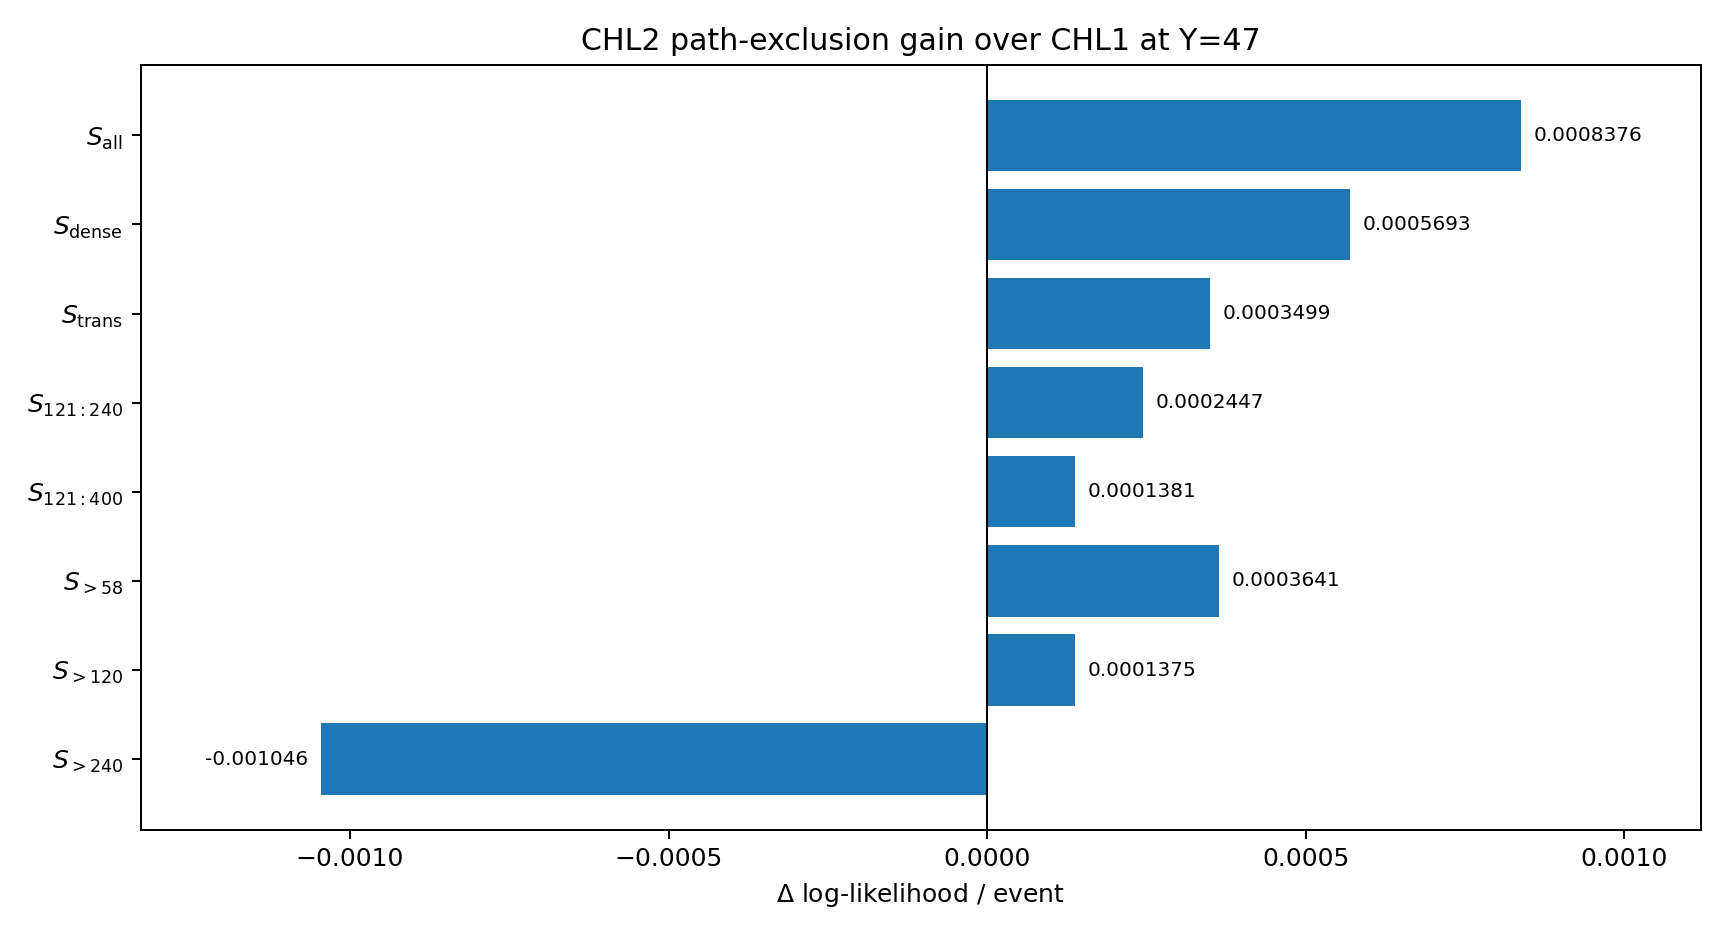
\includegraphics[width=0.94\textwidth]{figures/fig03_chl2_chl1_gain.png}
\caption{Per-event log-likelihood gain of CHL2 path-exclusion over CHL1 ratio-only.}\label{fig:chl2_gain}
\end{figure}

The zero-memory comparisons are part of the same likelihood audit.  Table~\ref{tab:memory_baselines} gives representative full-support values.  The large positive gains show that CHL2 is not merely a calibrated marginal gap distribution: removing dependence on the previous gap $g_1$ loses substantial likelihood.

\begin{table}[H]\centering\small
\begin{tabular}{lrr}
\toprule
Baseline & loglik/event in $S_{\rm all}$ & CHL2 gain \\
\midrule
HL2 order-zero & -3.442355 & 0.214227 \\
Mask-only order-zero & -3.498579 & 0.270451 \\
Cramer order-zero & -3.499383 & 0.271255 \\
Cramer--Granville order-zero & -3.446307 & 0.218180 \\
Cramer--Granville gap-exclusion order-zero & -3.651815 & 0.423687 \\
\bottomrule
\end{tabular}
\caption{Full-support memory-irreducibility checks.  Each row is a zero-memory baseline evaluated on the same DS1 support and common scale anchor.}\label{tab:memory_baselines}
\end{table}

\section{Cutoff stability}
The cutoff sweep recomputes the model for $Y\in\{31,47,61,73\}$.  A stable positive gain means that the path-exclusion improvement is not a visible artifact of a single truncation horizon.

\begin{empirical}[Cutoff stability]
For every principal stratum, the gain of CHL2 path-exclusion over CHL1 ratio-only remains positive for all four evaluated truncation horizons $Y\in\{31,47,61,73\}$.
\end{empirical}

\begin{table}[H]\centering\small
\begin{tabular}{lrrr}
\toprule
Stratum & min$_Y\Delta\ell$ & mean$_Y\Delta\ell$ & positive $Y$ \\
\midrule
$S_{\rm all}$ & 0.000819 & 0.000837 & 4/4 \\
$S_{\rm dense}$ & 0.000560 & 0.000567 & 4/4 \\
$S_{\rm trans}$ & 0.000338 & 0.000349 & 4/4 \\
$S_{121:240}$ & 0.000239 & 0.000269 & 4/4 \\
$S_{121:400}$ & 0.000124 & 0.000163 & 4/4 \\
$S_{>58}$ & 0.000350 & 0.000364 & 4/4 \\
$S_{>120}$ & 0.000124 & 0.000162 & 4/4 \\
$S_{>240}$ & -0.001095 & -0.001077 & 0/4 \\
\bottomrule
\end{tabular}
\caption{$Y$-sweep stability against CHL1.  The sparse $S_{>240}$ filter contains only $2{,}606$ events; its negative sign is reported for transparency but is not used for conclusions.}
\end{table}

\begin{figure}[H]\centering
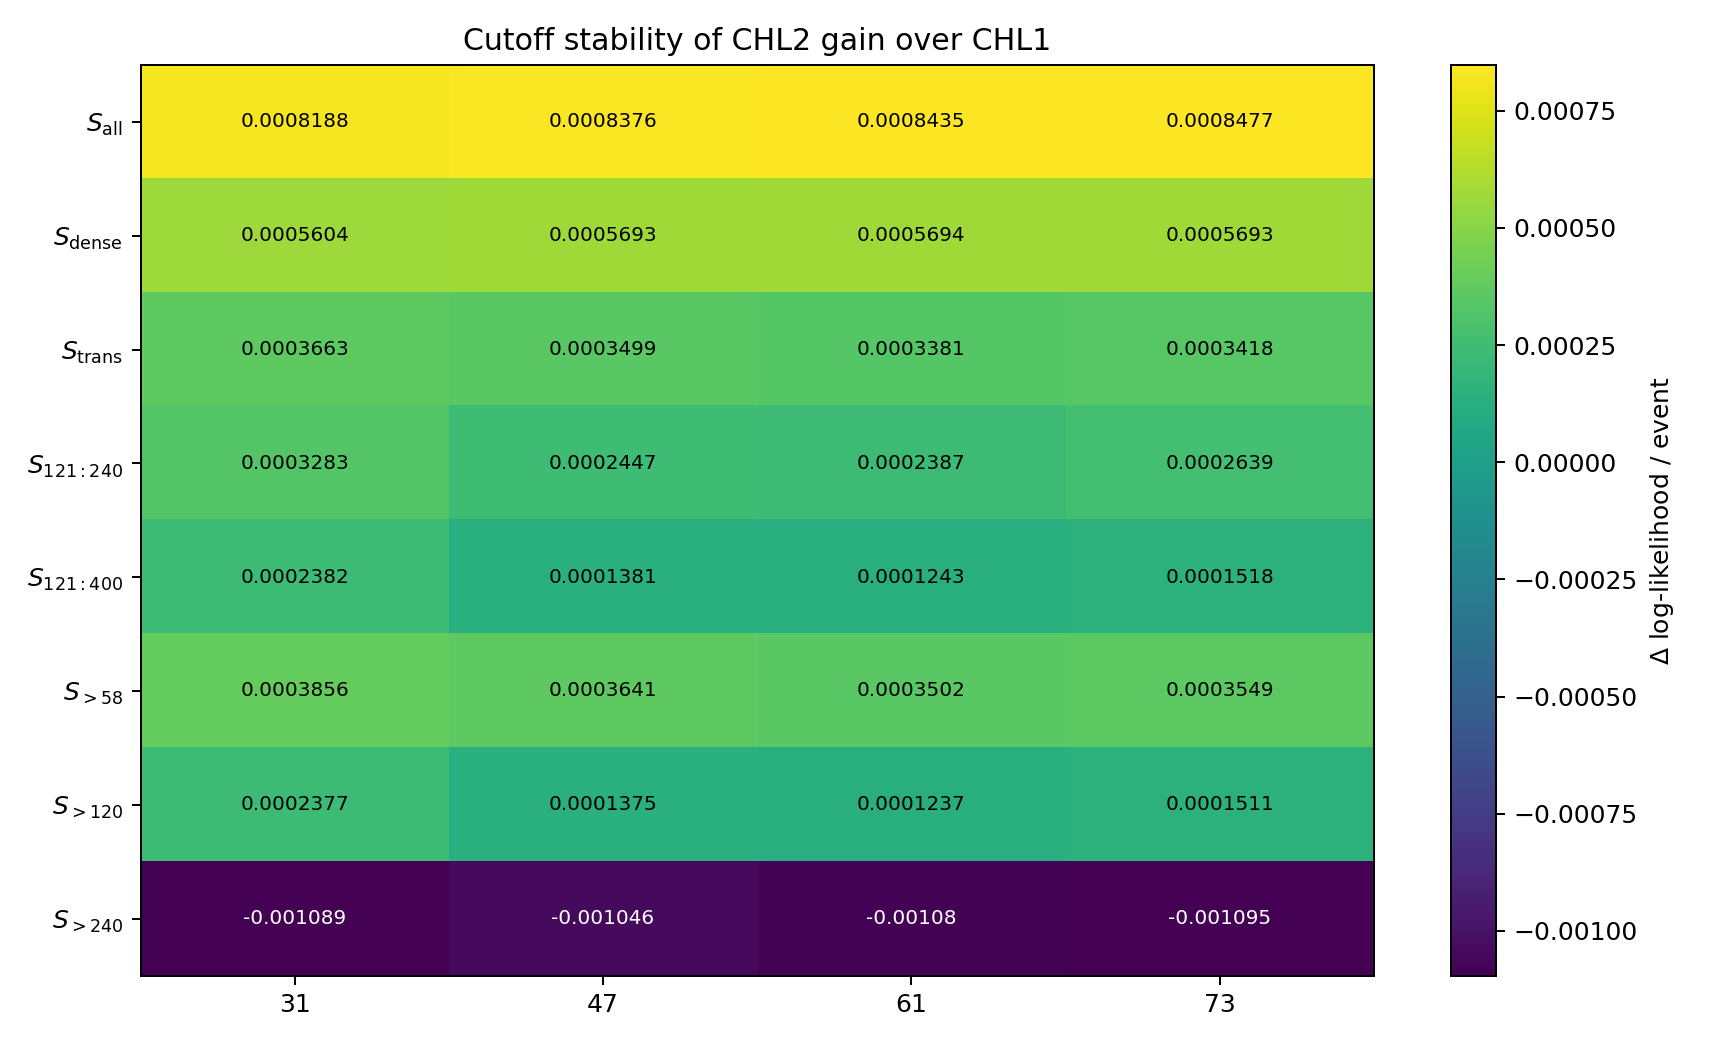
\includegraphics[width=0.86\textwidth]{figures/fig04_y_sweep_heatmap.png}
\caption{Cutoff stability heatmap of the CHL2-vs-CHL1 gain.}\label{fig:y_sweep_heatmap}
\end{figure}

\section{Orientation-lifted modular diagnostics}\label{sec:modular_diagnostics}
A prime-residue transition diagnostic should compare
\[
T_q(b,a)=P(p_n\equiv a\pmod q\mid p_{n-1}\equiv b\pmod q)
\]
over reduced residue classes.  A naive direct diagnostic, used as a negative control below, assigns gap-residue mass to transition rows without dividing by the number of valid oriented reduced-residue edges.  This diagnostic suggested a wrong-sign anomaly for $q=3$.  The orientation-lift audits showed that the anomaly was caused by this incomplete projection, not by the CHL2 gap kernel.

\subsection{Orientation lift}\label{sec:orientation_lift}
The modular diagnostic begins with the prime-residue transition matrix
\[
T_q(b,a)=P(p_n\equiv a\pmod q\mid p_{n-1}\equiv b\pmod q).
\]
A gap kernel does not directly output this matrix.  It outputs mass on gap residues
\[
p_r=P(g\equiv r\pmod q).
\]
To turn $p_r$ into a row-wise transition matrix, one must remember that a residue $r$ does not contribute independently to every row.  It contributes only to those reduced residue classes $b$ for which the oriented edge
\[
b\longrightarrow b+r\pmod q
\]
remains inside $(\mathbb Z/q\mathbb Z)^*$.  Thus the gap-residue population must first be lifted through the directed graph of valid reduced-residue edges.

Define
\[
N_r(q)=\#\{b\in(\mathbb Z/q\mathbb Z)^*: b+r\in(\mathbb Z/q\mathbb Z)^*\}.
\]
This is a combinatorial quantity attached to the directed Cayley graph of the reduced residue classes, with directed edges $b\to b+r$ whenever both endpoints remain reduced.  The edge multiplicity $N_r(q)$ is not introduced here as a new residue-counting fact.  Tao's exposition of the Lemke Oliver--Soundararajan bias already makes the relevant asymmetry transparent; for a prime modulus $p$, the diagonal gap residue $r\equiv0\pmod p$ has
\[
N_0(p)=p-1
\]
valid reduced starting classes, whereas a nonzero residue $r\not\equiv0\pmod p$ has
\[
N_r(p)=p-2.
\]
Holt's gap-population framework uses the same kind of counting to describe aggregate residue-class populations, addressing the inter-class distribution of gaps.  The present diagnostic operates in the complementary intra-class direction: given a model-produced gap-residue population, it specifies the uniform valid-edge projection from that population to a row-wise transition matrix.

The orientation-lifted matrix therefore distributes the mass $p_r$ over its $N_r(q)$ valid edges as $p_r/N_r(q)$ and then normalizes row-wise.  This lift is not a heuristic repair for modulus $3$, nor a claim of a new residue multiplicity.  It is the natural null intra-class projection associated with a gap kernel.  Equivalently, for each fixed residue class $r$, it is the maximum-entropy assignment on the valid edge set
\[
E_r(q)=\{(b,a):a\equiv b+r\pmod q,\ b,a\in(\mathbb Z/q\mathbb Z)^*\}
\]
subject only to the inter-class constraint
\[
\sum_{(b,a)\in E_r(q)} m_{b,a}=p_r.
\]
Any stable deviation from this uniform valid-edge assignment would itself be an intra-class signal beyond the gap-residue population.

The effect is most transparent in modulus $3$.  The reduced classes are $1$ and $2$.  The diagonal gap class $r=0$ has two valid oriented edges,
\[
1\to1,
\qquad
2\to2,
\]
so its mass must be split between two rows.  By contrast, the off-diagonal class $r=1$ has only the valid edge $1\to2$, because $2+1\equiv0\pmod3$ is not a reduced prime residue.  Similarly, $r=2$ has only the valid edge $2\to1$.  Therefore
\[
T(1,1)\propto p_0/2,
\qquad
T(1,2)\propto p_1,
\]
\[
T(2,2)\propto p_0/2,
\qquad
T(2,1)\propto p_2.
\]
The naive direct diagnostic missed this geometry and effectively allowed the diagonal mass $p_0$ to enter each row without being split.  In other words, it assigned the diagonal mass $p_0$ to each row instead of distributing it over the two valid diagonal edges, artificially doubling its contribution in the binary reduced space and creating the illusion of diagonal persistence.  The corrected behavior is shown in Figure~\ref{fig:orientation_lift_diag}: the orientation-lifted CHL2 diagnostic follows the empirical diagonal repulsion in $q=3$, while the naive direct diagnostic has the wrong sign.

\begin{proposition}[Orientation lift]
The row-wise transition matrix induced by a gap-residue population is obtained by distributing each residue class mass $p_r$ over valid reduced-residue oriented edges with weight $p_r/N_r(q)$ and then normalizing by row.  The naive assignment that places $p_r$ independently in every row overcounts edges and can create spurious diagonal persistence.
\end{proposition}
\subsection{Empirical correction of the modular diagnostic}
\begin{empirical}[Resolution of the apparent $q=3$ anomaly]
The naive direct diagnostic gives diagonal probability $0.521895$ for CHL2 in modulus $3$, while the empirical diagonal probability is $0.455612$.  After orientation lift, the CHL2 diagonal probability is $0.455864$, with the correct diagonal-repulsion sign.  The improvement is not merely cosmetic: in $q=3$ the KL divergence falls from $8.8\times10^{-3}$ to $4.0\times10^{-7}$, and the same oriented construction improves every audited modulus.  Table~\ref{tab:orientation_lift_diag} and Figure~\ref{fig:orientation_lift_diag} summarize the correction across the audited moduli.
\end{empirical}

\begin{table}[H]\centering\small
\begin{tabular}{rrrrrr}
\toprule
$q$ & empirical diag & naive direct CHL2 & oriented CHL2 & KL naive & KL oriented \\
\midrule
3 & 0.455612 & 0.521895 & 0.455864 & 0.008796 & $4.03\times10^{-7}$ \\
5 & 0.192411 & 0.236276 & 0.192115 & 0.005937 & 0.000309 \\
7 & 0.111342 & 0.130993 & 0.111982 & 0.002078 & 0.000268 \\
11 & 0.051379 & 0.100000 & 0.051514 & 0.040355 & 0.000355 \\
13 & 0.036536 & 0.083333 & 0.036504 & 0.053835 & 0.000366 \\
\bottomrule
\end{tabular}
\caption{Naive direct modular diagnostic versus orientation-lifted CHL2.  The naive direct diagnostic is the failing projection; the orientation-lifted diagnostic distributes gap-residue mass over valid directed reduced-residue edges and improves every audited modulus.  The round naive diagonal values for $q=11$ and $q=13$ coincide with $1/(q-1)$ in this audit, reflecting the near-uniform reduced-residue diagonal produced by the naive direct projection before valid-edge correction.}\label{tab:orientation_lift_diag}
\end{table}

\begin{figure}[H]\centering
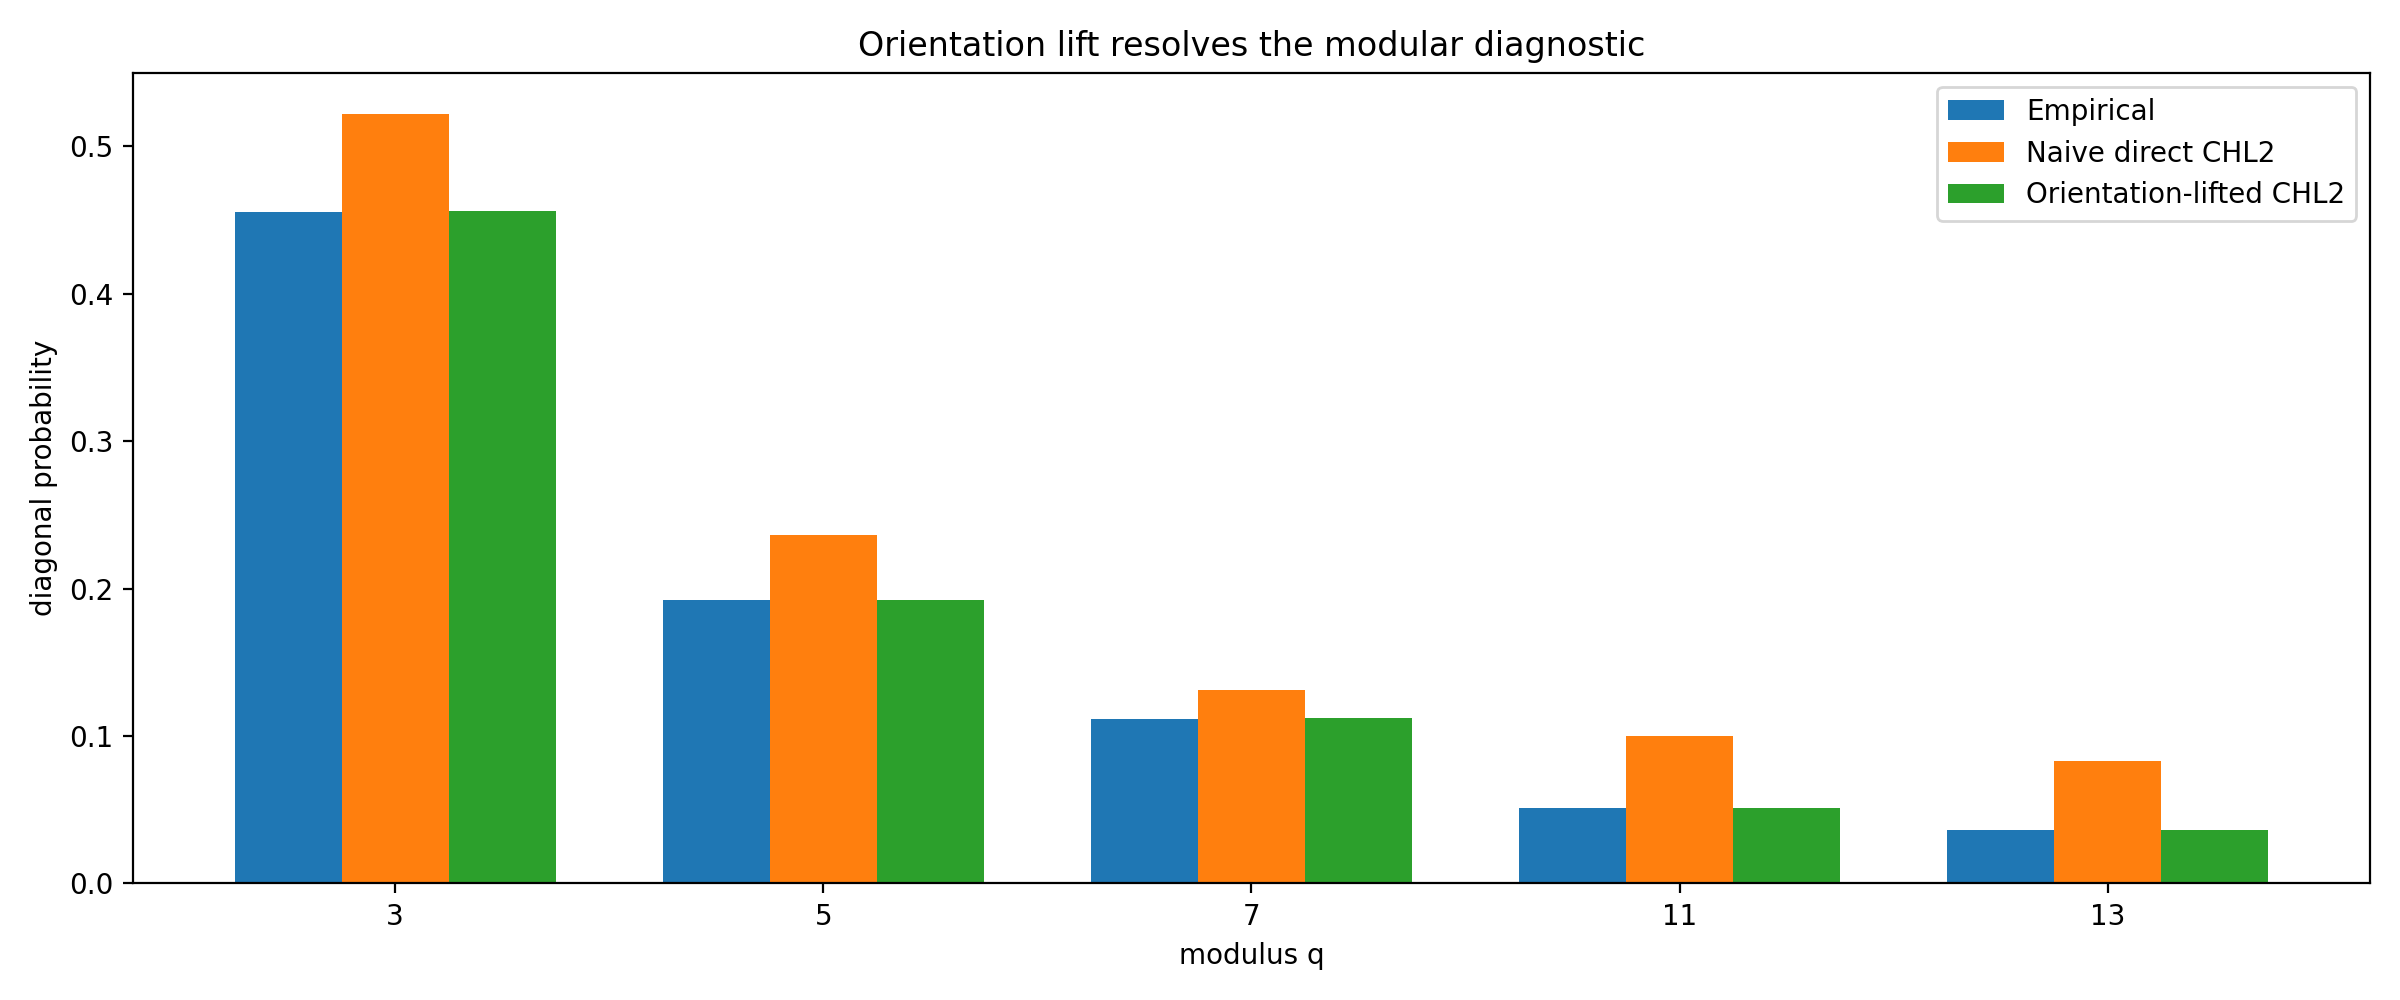
\includegraphics[width=0.92\textwidth]{figures/fig05_orientation_lift_diag.png}
\caption{Empirical diagonal probabilities, naive direct CHL2, and orientation-lifted CHL2.  The naive direct diagnostic visibly misses the diagonal probabilities, while the oriented diagnostic nearly overlaps the empirical bars.}\label{fig:orientation_lift_diag}
\end{figure}

\subsection{The scale wave in the gap population}\label{sec:scale_wave}
The gap-residue population has its own scale structure.  In DS1 the modulo-$3$ gap-population log-odds
\[
D_3^{\rm gap}=2\log\frac{P(g\equiv0\pmod3)}{1-P(g\equiv0\pmod3)}
\]
changes sign across gap regimes: strong repulsion at small gaps, persistence at mid-range gaps, and a weaker return to repulsion in the long tail.  The factor $2$ comes from converting the gap-residue odds into the two-row diagonal/off-diagonal log-odds of the binary reduced-residue system under the observed symmetry $P(g\equiv1\pmod3)\approx P(g\equiv2\pmod3)$; the empirical pair-count tables record that the basic off-diagonal gaps $g=2$ and $g=4$ are nearly perfectly balanced.  Under this symmetric compression, both diagonal cells carry the same gap-residue mass after orientation lift.  Figure~\ref{fig:scale_wave} is meant to be read as part of the argument: the modular flow is not a monotone decay toward zero, but a genuine scale wave.  CHL2 reproduces this wave closely at the gap-population level because the path factor $\Omega_Y^{\mathrm{path}}$ does not merely see the length of a proposed gap; it sums the conditional intensities of possible interior prime positions after the endpoints are fixed.  This is also why CHL2 is stronger than a Cramer--Granville order-zero baseline: it sees the conditional texture of the interval, not only its exponential length scale.  With that gap population in place, the orientation lift resolves the modular diagnostic without altering the gap kernel.

\begin{figure}[H]\centering
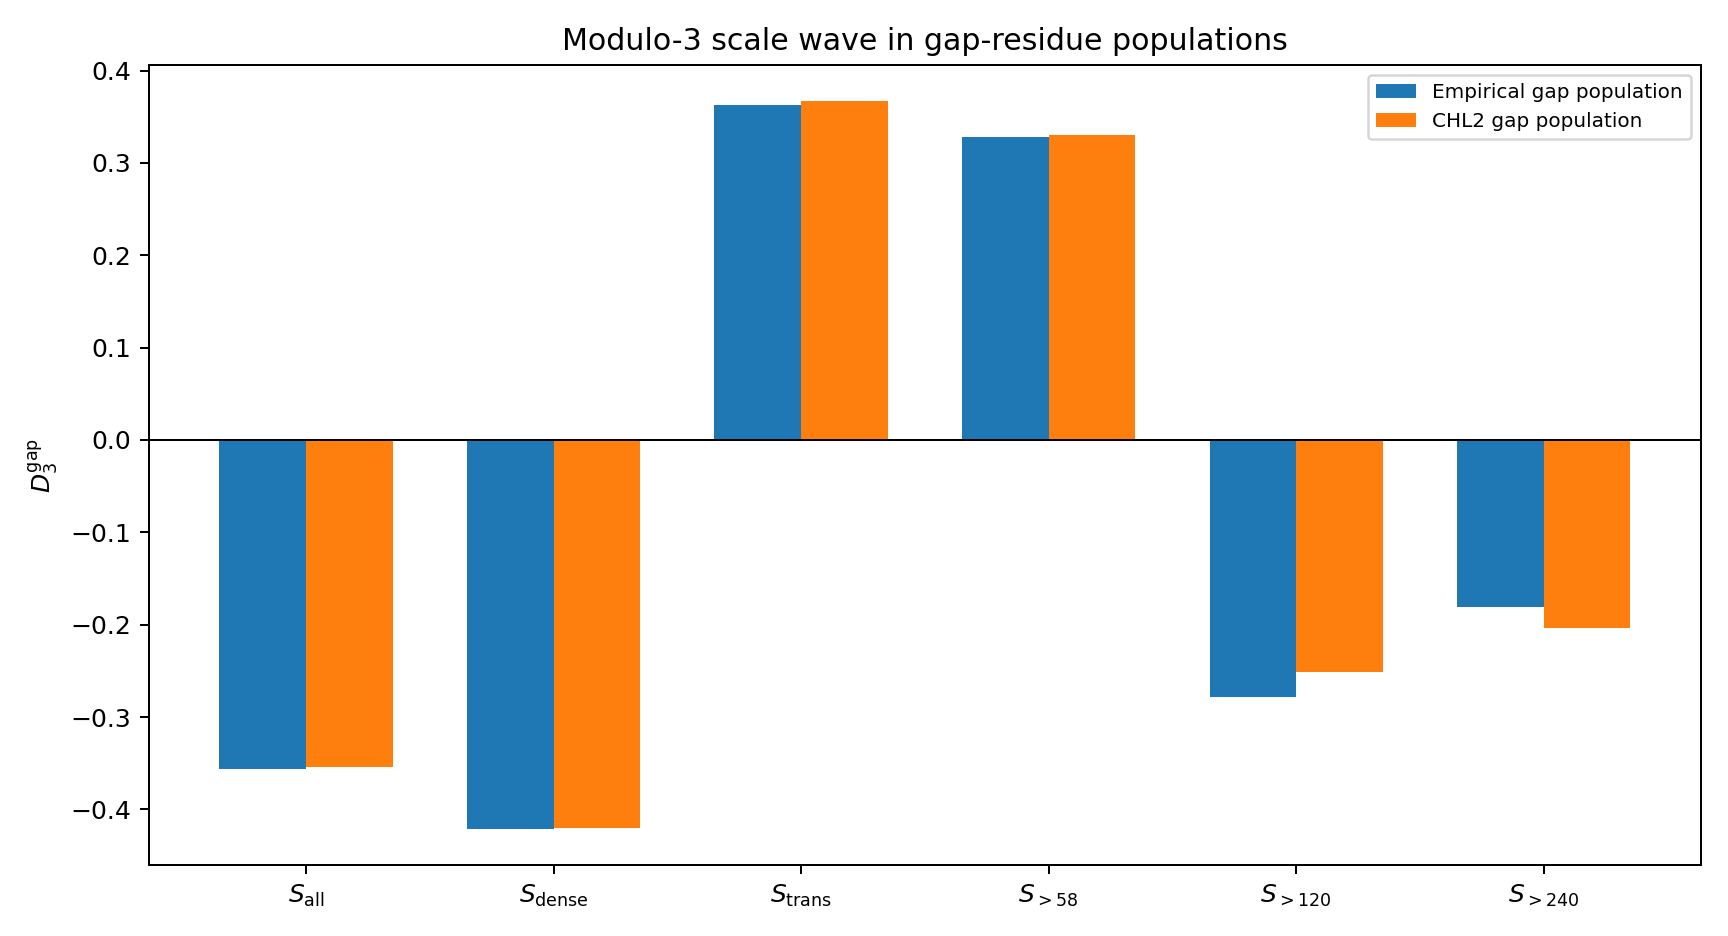
\includegraphics[width=0.92\textwidth]{figures/fig06_scale_wave.png}
\caption{The modulo-$3$ scale wave in the empirical and CHL2 gap-residue populations.}\label{fig:scale_wave}
\end{figure}

\section{Negative controls and model refinement}
The final CHL2 construction is not the first model that was tried.  Several alternatives were natural, and each would have led to a plausible but weaker story if it had not been tested directly.  We include these negative controls because they explain the shape of the final kernel: CHL2 is not a collection of convenient factors, but the remainder after simpler or more tempting explanations were eliminated.

\subsection{Limits of empirical geometry}
The earliest experimental models used low-dimensional geometric features of consecutive gaps, such as shape, balance, and tail scale.  These features were useful as exploratory coordinates: they revealed that the pair $(g_1,g_2)$ is not well described by a gap-size marginal alone.  They also helped identify the path-memory nature of the problem.

However, the empirical geometry had a serious weakness.  Its coefficients were not forced by a classical arithmetic object.  Once the conditional Hardy--Littlewood ratio
\[
R_Y(g_2\mid g_1)=\frac{\SY(H_3)}{\SY(H_2)}
\]
was introduced, much of the apparent geometric structure was absorbed by the singular-series conditioning itself.  In other words, the geometry was a good laboratory lens, but not a satisfactory final foundation.  It was therefore downgraded to historical precursor status rather than retained as a core factor in the paper.

\subsection{The inadequacy of higher-order low-wheel clusters}\label{sec:second_order_control}
A second natural objection concerns the first-order Poisson approximation in the no-interior survival factor.  If CHL2 appeared to fail in the two-state reduced-residue system modulo $3$, the most compressed low-wheel case, perhaps the problem was that $\Omega_Y^{\mathrm{path}}$ ignored pairwise dependencies among possible interior primes.  This led to a second-order low-wheel negative-control experiment, detailed in the supplementary computational archives.

For two interior candidates $u<v$, one can form the quintic tuple
\[
H_5(u,v)=\{0,g_1,g_1+u,g_1+v,g_1+g_2\}.
\]
In this negative-control experiment we set
\[
p_u=I_Y(u\mid g_1,g_2;x)=\frac{1}{\log x}\frac{\SY(H_4(u))}{\SY(H_3)},
\]
and
\[
p_{uv}=\frac{1}{(\log x)^2}\frac{\SY(H_5(u,v))}{\SY(H_3)}.
\]
The pair cumulant is
\[
\kappa_{uv}=p_{uv}-p_up_v,
\]
and the corresponding second-order intensity, with $\Omega_Y^{(1)}\equiv\Omega_Y^{\rm path}$, has the form
\[
\Omega_Y^{(2)}=\Omega_Y^{(1)}-\sum_{u<v}\kappa_{uv}.
\]
This correction behaves algebraically as expected.  When the low-wheel quintic tuple becomes inadmissible, it produces a hard zero and a negative cumulant, increasing the no-interior intensity.  The experiment therefore confirmed that the code and the arithmetic mechanism were detecting genuine low-wheel exclusions.

But the correction did not remove the naive direct $q=3$ sign error.  Negative hard-zero cumulants were largely offset by positive cumulants from compatible residue configurations.  This failure was informative: the apparent modular anomaly was not caused primarily by missing second-order interior-prime exclusions.  It pointed away from the no-interior survival factor and toward the way gap-residue mass was being lifted into a residue-transition matrix.

\begin{table}[H]\centering\small
\begin{tabular}{lrl}
\toprule
Diagnostic & predicted diagonal & status \\
\midrule
\multicolumn{3}{l}{Empirical $q=3$ diagonal target: $0.455612$.}\\
\midrule
Naive direct CHL2 & 0.521895 & wrong sign \\
Second-order low-wheel cumulant & $\approx0.5216$ & wrong sign \\
\bottomrule
\end{tabular}
\caption{Negative-control summary for the second-order low-wheel cumulant.  The empirical diagonal probability is shown as the fixed target; both tested diagnostics remained above the threshold $0.5$ and therefore retained the wrong sign.}
\end{table}

\subsection{Residual spectral corrector}
Before the orientation-lift defect was isolated, another natural diagnostic was to fit a rank-one residual corrector for $q=3$.  For the two reduced classes $1,2$, define the signed diagonal mode
\[
K_3=\begin{pmatrix}1&-1\\-1&1\end{pmatrix}.
\]
For modulus $3$ there is a single non-principal Dirichlet character $\chi$ with $\chi(1)=1$ and $\chi(2)=-1$, and $K_3(b,a)=\chi(b)\chi(a)$ is precisely the diagonal/off-diagonal character mode.  A positive coefficient on this mode means diagonal persistence; a negative coefficient means diagonal repulsion.

For the naive direct diagnostic, let
\[
\mathcal R(b,a)=\log\frac{T_3^{\rm emp}(b,a)+\varepsilon}{T_3^{\rm naive}(b,a)+\varepsilon}
\]
and subtract the mean of each row to obtain the row-centered residual $\widetilde{\mathcal R}$.  The audit used the unweighted Frobenius projection
\[
\theta_3=\frac{\langle \widetilde{\mathcal R},K_3\rangle_F}{\langle K_3,K_3\rangle_F}.
\]
For a $2\times2$ row-centered transition residual this is equivalent to
\[
\theta_3=\frac{D_3(T^{\rm emp})-D_3(T^{\rm naive})}{4}.
\]
The fitted residual coefficient for the naive direct diagnostic was about $\theta_3=-1.33\times10^{-1}$ and corrected the sign.  It was not retained as a new arithmetic force because the later orientation-lift audit showed that the coefficient was compensating a projection error: once gap-residue mass is lifted through valid directed edges, the rank-one correction is no longer needed.

\subsection{Truncated LOS projections}
A third natural route was to use the Oliver--Soundararajan phenomenon more directly.  Since their work concerns biases in consecutive prime residue classes, it was natural to ask whether a local truncated LOS projection could generate the missing $q=3$ transfer term.  We tested this by projecting low-order Hardy--Littlewood cluster contributions onto the diagonal/off-diagonal character mode.

This test again produced a useful negative result.  For $q=3$, the reduced classes are $1$ and $2$, and the signed diagonal/off-diagonal mode is the matrix $K_3$ above.  Equivalently, if $T$ is row-stochastic, the diagonal log-odds
\[
D_3(T)=\log\frac{T(1,1)T(2,2)}{T(1,2)T(2,1)}
\]
measures diagonal persistence or repulsion.  This matrix log-odds is denoted differently from the gap-population statistic $D_3^{\rm gap}$ in Section~\ref{sec:scale_wave} to emphasize that the former is computed from a transition matrix and the latter from a gap-residue population.  The local LOS projection tested here was obtained by projecting low-order Hardy--Littlewood cluster contributions onto this signed mode; it did not attempt to reproduce the full secondary-term theory of Lemke Oliver--Soundararajan \cite{lemke-sound-secondary}.  It detected the correct non-principal character mode, but its amplitude was much too small: the empirical residual coefficient is of order $-1.3\times10^{-1}$, while the truncated local projection produced a coefficient of order $-10^{-3}$.  Thus the projection pointed in the right direction but could not explain the observed diagonal repulsion.

\begin{table}[H]\centering\small
\begin{tabular}{lrr}
\toprule
Quantity & empirical / required & local LOS projection \\
\midrule
Dominant $q=3$ residual character coefficient & $\approx -1.33\times10^{-1}$ & $\approx -1.3\times10^{-3}$ \\
Sign of projected contribution & negative & negative \\
Amplitude relative to requirement & 1.0 & $\approx 10^{-2}$ \\
\bottomrule
\end{tabular}
\caption{Negative-control summary for the local LOS projection.  The mode was correct but the projected amplitude was roughly two orders of magnitude too small.}
\end{table}

These negative controls are summarized in Table~\ref{tab:negative_controls} and Figure~\ref{fig:negative_controls}.  They are not failures of the project; they are the reason the final paper distinguishes carefully between the CHL2 gap-survival kernel and the orientation-lifted modular diagnostic.

\begin{table}[H]\centering\small
\begin{tabularx}{\textwidth}{lXX}
\toprule
Route & Why it was natural & Outcome \\
\midrule
Empirical Shape/Balance/Tail & Early path geometry features captured visible structure. & Degraded to historical precursor after conditional singular-series ratios removed fitted degrees of freedom. \\
Second-order low-wheel clusters & Natural correction to first-order Poisson no-interior survival. & Detected hard-zero quintic configurations but did not resolve the naive direct $q=3$ diagnostic. \\
Local LOS projection & Directly related to biases in consecutive primes. & Detected the correct character mode but with insufficient amplitude. \\
Residual spectral $\theta_3$ & A rank-one corrector fixed the naive direct $q=3$ sign. & Later identified as compensating an orientation-lift defect, not as a new core force. \\
Orientation lift & Respects valid reduced-residue directed edges. & Corrects $q=3$ and improves $q=5,7,11,13$ diagnostics. \\
\bottomrule
\end{tabularx}
\caption{Negative controls and refinement path.}\label{tab:negative_controls}
\end{table}

\begin{figure}[H]\centering
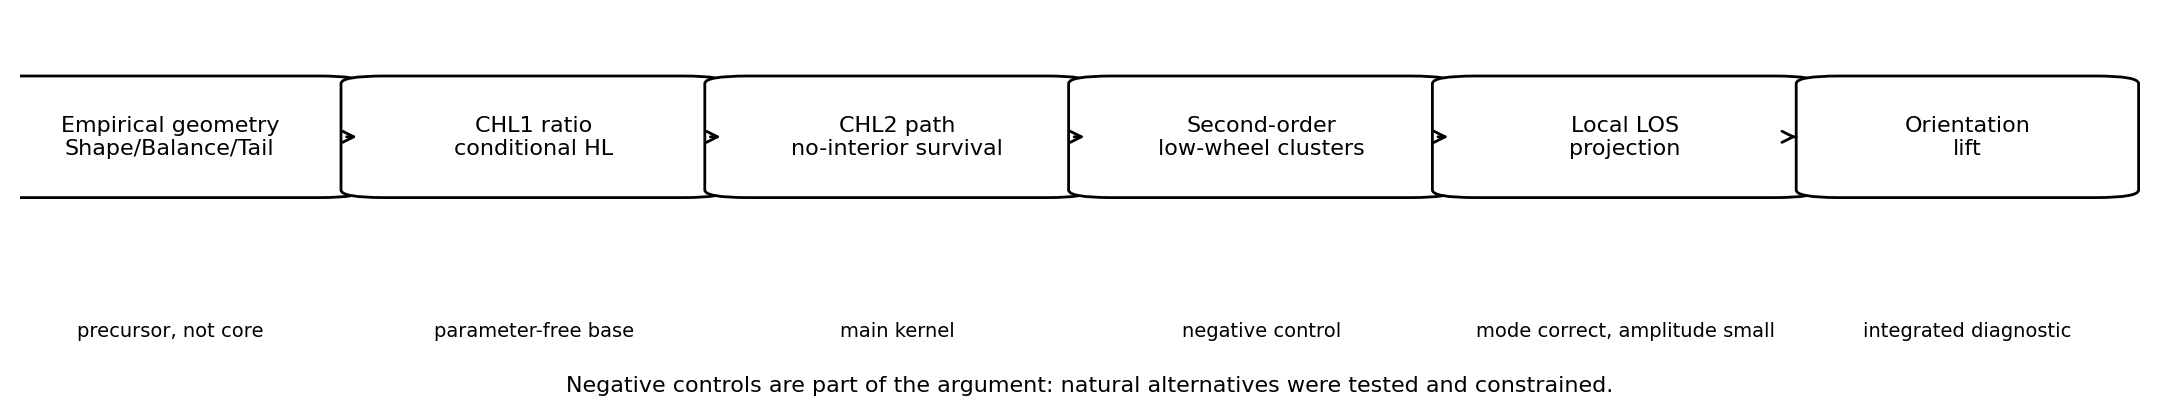
\includegraphics[width=0.98\textwidth]{figures/fig07_negative_controls.png}
\caption{Schematic refinement path and negative controls.}\label{fig:negative_controls}
\end{figure}


\section{Logical dependency map}
\begin{table}[H]\centering\scriptsize
\begin{tabularx}{\textwidth}{>{\raggedright\arraybackslash}p{0.24\textwidth}>{\raggedright\arraybackslash}p{0.38\textwidth}>{\raggedright\arraybackslash}p{0.30\textwidth}}
\toprule
Claim & Depends on & Audit evidence \\
\midrule
CHL1 conditional kernel & Singular-series ratio $\SY(H_3)/\SY(H_2)$ & Formula and finite support. \\
CHL2 path correction & Conditional $H_4/H_3$ no-interior intensity & Likelihood and pairwise-gain audit. \\
Cutoff stability & Recomputed kernels for $Y=31,47,61,73$ & $Y$-sweep audit. \\
Memory irreducibility & Conditional kernels compared with order-zero baselines & Memory-irreducibility audit. \\
Orientation lift resolves the apparent $q=3$ anomaly & Gap-residue population plus valid-edge row projection & Orientation-lifted modular audit. \\
The naive direct diagnostic is a negative control & It assigns gap-residue mass to rows without valid-edge normalization & Oriented-versus-naive modular comparison. \\
Second-order low-wheel clusters were not the cause & Quintic hard-zero cumulants failed to cross the $q=3$ diagonal threshold & Supplementary negative-control archive. \\
Truncated local LOS projection was too weak & It found the correct character mode but not the observed amplitude & LOS-projection negative-control audit. \\
\bottomrule
\end{tabularx}
\caption{Logical dependency map for the principal claims and the audit evidence supporting them.  The exact script-to-output mapping is given in the reproducibility section.}
\end{table}


\section{Limitations}
The results are finite-window computational audits, not asymptotic theorems.  The truncation horizon $Y$ is finite, the support is finite, and the scale $\log x$ is treated as locally constant on DS1.  The no-interior survival factor is first-order Poisson.  The orientation lift corrects the modular diagnostic layer; it does not turn CHL2 into a proof of any open prime conjecture.

The sparse $S_{>240}$ stratum is retained only as a stress diagnostic.  It contains $2{,}606$ events in DS1, its scores are renormalized on a very small filtered support, and its signs are not used in any principal conclusion.

The orientation lift should also be interpreted carefully.  It is the null intra-class assignment associated with a gap-residue population.  It distributes mass uniformly over valid directed reduced-residue edges.  It is not a complete model of every possible intra-class bias after the lift; any stable residual after this projection would define a new problem.

Finally, the negative controls described above are finite computational audits.  The second-order low-wheel cluster experiment rules out the tested pairwise no-interior correction as the source of the naive direct $q=3$ anomaly.  The local LOS projection rules out the simple truncated projection tested here, not the full secondary-term theory of Lemke Oliver--Soundararajan.


\section{Reproducibility}
The repository contains four layers: data generation, the importable mathematical kernel, paper audits, and research tools.  Runtime telemetry is written by the main scripts and records elapsed time, command line, CPU count, truncation horizon, block counts, output-row counts, and modular diagnostic status.

\begin{figure}[H]\centering
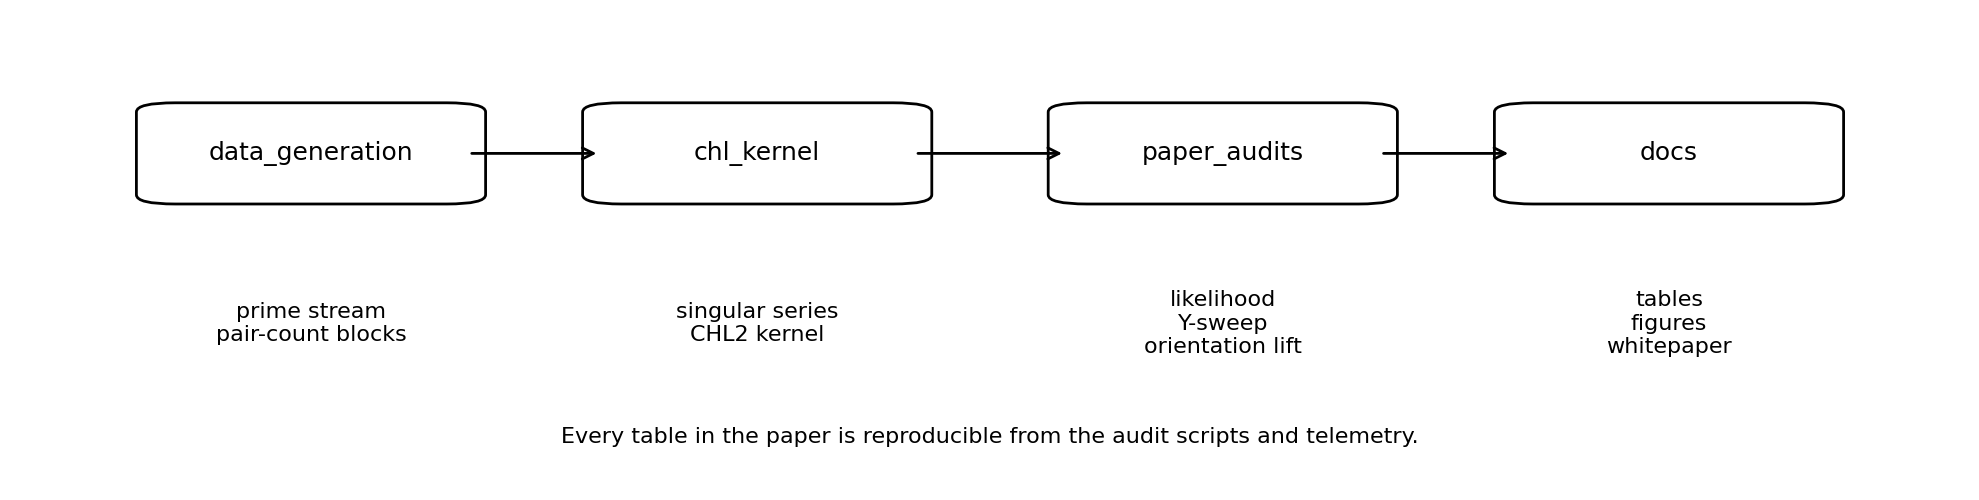
\includegraphics[width=0.86\textwidth]{figures/fig08_repro_pipeline.png}
\caption{Reproducibility architecture of the repository.}\label{fig:repro_pipeline}
\end{figure}

The main scripts associated with the tables and figures are:
\begin{center}\scriptsize
\begin{tabularx}{\textwidth}{>{\raggedright\arraybackslash}p{0.30\textwidth}>{\raggedright\arraybackslash}X}
\toprule
Output in paper & Script and primary files \\
\midrule
Likelihood results, Table 1 and Figure~\ref{fig:chl2_gain} & \path{paper_audits/chl2_consecutive_exclusion_audit.py}; outputs \path{chl2_conditional_summary.csv}, \path{chl2_pairwise_gains.csv}. \\
$Y$-sweep stability table and Figure~\ref{fig:y_sweep_heatmap} & \path{paper_audits/chl2_y_sweep.py}; outputs \path{chl2_y_sweep_stability.csv}, \path{chl2_y_sweep_gains.csv}. \\
Orientation-lifted modular diagnostic, Table~\ref{tab:orientation_lift_diag} and Figure~\ref{fig:orientation_lift_diag} & \path{paper_audits/chl4d5_orientation_lift_os_replacement.py}; outputs \path{chl2_os_old_direct_vs_oriented.csv} and \path{chl2_os_oriented_prime_residue_summary.csv}. \\
Scale-wave diagnostic, Figure~\ref{fig:scale_wave} & \path{paper_audits/chl4d2_gap_population_bias_audit.py}; output \path{chl4d2_scale_wave_summary.csv}. \\
Negative controls & Supplementary computational audit scripts; the paper reports only the summaries needed to explain why they were not retained. \\
\bottomrule
\end{tabularx}
\end{center}

Core commands for a fresh check are:
\begin{verbatim}
python -m compileall .
python tests/test_kernel_smoke.py
python paper_audits/chl2_consecutive_exclusion_audit.py ...
python paper_audits/chl2_y_sweep.py ...
python paper_audits/chl4d5_orientation_lift_os_replacement.py ...
\end{verbatim}
The DS1 runtime telemetry records the number of workers, elapsed time, and output-row counts.  On ordinary multicore hardware, the principal audits run in minutes rather than days.

\section{Conclusion}
CHL2 is a conditional Hardy--Littlewood Markov kernel for consecutive prime gaps.  The model is obtained by conditioning the singular series, adding a first-order no-interior survival factor, and normalizing over even admissible candidate gaps.  It improves CHL1 in the DS1 audit and remains stable across the tested truncation horizons.

The major modular change in this release is that the apparent $q=3$ failure was traced to the naive direct diagnostic lift, not to the CHL2 gap kernel.  Once gap-residue populations are lifted through valid oriented reduced-residue edges, CHL2 reproduces the empirical diagonal repulsion in $q=3$ and improves the modular diagnostics for all audited moduli.  This strengthens the core CHL2 claim while keeping the scope narrow: a finite reproducible conditional kernel, not an asymptotic theorem.

\appendix
\section{Orientation-lift details}
For a modulus $q$, let $G_q=(\mathbb Z/q\mathbb Z)^*$ and let $p_r=P(g\equiv r\pmod q)$.  The directed edges associated with $r$ are
\[
E_r(q)=\{(b,a)\in G_q^2: a\equiv b+r\pmod q\}.
\]
Their number is $N_r(q)=|E_r(q)|$.  The orientation lift puts mass $p_r/N_r(q)$ on each edge in $E_r(q)$ and then normalizes by row.  If $N_r(q)=0$, the residue class $r$ contributes no reduced-residue transition.

The geometric explanation of the $q=3$ case was given in the main text because it is central to the modular diagnostic.  This appendix records the general construction: for every residue $r$, the mass $p_r$ is divided by the number of valid directed reduced-residue edges before row normalization.  The naive direct diagnostic failed because it implicitly skipped this edge-counting step.


\section{Scale anchoring and first-order survival details}\label{app:maxent-poisson}
This appendix records two standard finite-support reductions used in the kernel definitions.  First, suppose the arithmetic part of a row gives nonnegative weights $w(h)$ on a finite even support $\mathcal G$.  Among distributions of the form obtained by exponentially tilting these weights and imposing a target mean $m$, the maximum-entropy/Lagrange-multiplier calculation gives
\[
P_\eta(h)=\frac{w(h)e^{\eta h}}{Z(\eta)},
\qquad
Z(\eta)=\sum_{h\in\mathcal G}w(h)e^{\eta h}.
\]
The mean is
\[
\mathbb E_\eta[h]=\frac{d}{d\eta}\log Z(\eta),
\]
and
\[
\frac{d}{d\eta}\mathbb E_\eta[h]=\operatorname{Var}_\eta(h)\ge0.
\]
Thus, on a non-degenerate finite support, the mean is monotone in $\eta$ and the scale-anchoring equation has a unique numerical solution.  In the DS1 audits the same one-scalar anchoring rule is given to every model, block, and stratum; it is a common scale constraint, not a CHL2-specific fit.

Second, the no-interior survival factor uses the first-order rare-event approximation.  If the possible interior positions have conditional intensities $I_Y(u\mid g_1,g_2;x)$ and are treated as weakly dependent rare events, then the total number of interior primes is approximated by a Poisson random variable with mean
\[
\Omega_Y^{\rm path}=\sum_u I_Y(u\mid g_1,g_2;x).
\]
The probability of observing no interior prime is then
\[
P(0\ \text{interior primes})\approx e^{-\Omega_Y^{\rm path}}.
\]
The second-order low-wheel negative control described in Section~\ref{sec:second_order_control} tested whether pairwise corrections to this first-order approximation were responsible for the naive modular diagnostic failure; they were not.

\section{Forward-looking remarks}
The results above close the finite-window audit of the CHL2 kernel and its orientation-lifted modular diagnostic.  They also suggest several natural continuations.  First, the orientation lift supplies a null intra-class assignment associated with a gap-residue population; any stable deviation after this lift would define a genuine residual intra-class bias.  A systematic benchmark of this residual across CHL2, Cramer--Granville, LOS-type projections, and Holt-style population models is a natural future project.  The following remarks are deliberately separated from the main empirical claims.  They are not proved in this paper and should be read as research directions enabled by the parameter-free structure of the kernel.

\subsection{Algorithmic use: CHL2 as a parameter-free search oracle}
The CHL2 kernel is inexpensive to evaluate once the finite singular-series factors and no-interior intensities have been cached.  This makes it useful beyond retrospective likelihood audits.  Given a current prime scale $x$, a previous gap $g_1$, and a candidate next gap $g_2$, the structural part of the negative log-weight is
\[
\mathcal C_Y(g_2\mid g_1;x)
=
-\log R_Y(g_2\mid g_1)+\Omegapath(g_1,g_2;x).
\]
Lower values of $\mathcal C_Y$ correspond to candidates favored by the conditional singular-series ratio and by the no-interior survival factor.  This score does not replace primality testing.  Instead, it supplies a parameter-free ordering of candidates before expensive verification is attempted.

A practical benchmark for this use case is a Hit@$K$ test, a standard retrieval-style metric in which success means that a target event appears among the first $K$ ranked candidates.  For each state $(g_1,x)$, one ranks admissible candidates $g_2$ by increasing $\mathcal C_Y$ and asks whether rare target events---large gaps, unusual constellations, or specified residue patterns---appear among the first $K$ candidates more often than under Cramer--Granville, uniform-admissible, or marginal Hardy--Littlewood baselines.  This turns the CHL2 kernel into a reproducible search oracle: the mathematical object remains the same as in the paper, while the evaluation criterion changes from likelihood to prioritized discovery.

The repository includes a prototype of this idea in the Hit@$K$ oracle.  Its role is exploratory.  A successful Hit@$K$ improvement would not by itself imply an asymptotic theorem, but it would make CHL2 useful as a computational guide for finding rare prime-gap configurations with fewer primality tests.

\subsection{Variational bridge to adaptive sieve weights}
A second direction is theoretical.  Classical Selberg--GPY--Maynard weights are designed to detect prime-rich admissible configurations \cite{selberg,gpy,maynard-small}.  CHL2 supplies a different object: a conditional target distribution for the next gap, depending on the previous gap and local scale.  It is therefore natural to ask whether CHL2 can be used as a variational target for adaptive sieve weights.

Let $w_\lambda(h)$ be a family of sieve weights on admissible candidate gaps.  A normalized sieve-induced distribution could be defined by
\[
P_{\mathrm{sieve},\lambda}(h\mid g_1,x)
=
\frac{w_\lambda(h)^2\,\mathbf 1_{\mathrm{adm}}(h)}
{\sum_k w_\lambda(k)^2\,\mathbf 1_{\mathrm{adm}}(k)}.
\]
One possible objective is then
\[
J(\lambda)
=
D_{\mathrm{KL}}\!\left(P_{\mathrm{sieve},\lambda}(\cdot\mid g_1,x)\,\Vert\,P_{\mathrm{CHL2}}(\cdot\mid g_1,x)\right)
+
\kappa\sum_d\frac{\lambda_d^2}{d}.
\]
This asks for sieve weights whose induced distribution is close to the CHL2 transition law, subject to a regularization term reminiscent of quadratic sieve energies.  In a first-order linearization one is led heuristically to coefficients of the form
\[
\lambda_d^{(1)}
\propto
\mu(d)\,
\mathbb E_{h\sim \mathrm{adm}}
\left[
\log\frac{1}{P_{\mathrm{CHL2}}(h\mid g_1,x)}\,\middle|\,d\mid h
\right].
\]
This formula is a conjectural linearization, not an optimality theorem.  Its purpose is to indicate how a CHL2 transition cost might be converted into a sieve-weight design problem.

If such a programme can be made analytic, it could potentially connect the conditional kernel studied here with modern multidimensional sieve weights.  In particular, one could ask whether the effective sieve level should become local,
\[
R\longrightarrow R(g_1,x),
\]
so that the weight adapts to the previous gap and to the no-interior path intensity.  This is a forward-looking bridge to Maynard--Tao-style sieve functionals, not a claim that CHL2 presently improves any known asymptotic bound.  The contribution of the present paper is to provide the finite conditional target distribution; developing an analytic adaptive-sieve theory from it remains open.

\section{AI-assisted workflow disclosure}
The author used AI-assisted systems, including ChatGPT, Gemini, and related tools, as interactive research assistants during exploratory, coding, diagnostic, and drafting phases.  Their use included code prototyping, debugging, construction of diagnostic tests, adversarial critique of hypotheses, summarization of numerical outputs, and drafting support.  All experiments were executed locally by the author.  All reported claims, mathematical formulations, code selections, and interpretations were reviewed and curated by the author, who assumes full responsibility for the manuscript.  No AI system is listed as an author.

\begin{thebibliography}{99}
\bibitem{cramer1936} H. Cramer, \emph{On the order of magnitude of the difference between consecutive prime numbers}, Acta Arithmetica \textbf{2} (1936), 23--46.
\bibitem{gpy} D. A. Goldston, J. Pintz, and C. Y. Yildirim, \emph{Primes in tuples I}, Annals of Mathematics \textbf{170} (2009), 819--862.
\bibitem{granville1995} A. Granville, \emph{Harald Cramer and the distribution of prime numbers}, Scandinavian Actuarial Journal \textbf{1995} (1995), 12--28.
\bibitem{hardy-littlewood} G. H. Hardy and J. E. Littlewood, \emph{Some problems of Partitio Numerorum III}, Acta Mathematica \textbf{44} (1923), 1--70.
\bibitem{holt2016} F. B. Holt, \emph{On the last digits of consecutive primes}, arXiv:1604.02443, 2016.
\bibitem{holt2024} F. B. Holt, \emph{Expected biases in the distribution of consecutive primes}, arXiv:2405.03540, 2024.
\bibitem{lau2024} C. F. Lau, \emph{Residue class patterns of consecutive primes}, arXiv:2409.12819, 2024.
\bibitem{lemke-sound} R. J. Lemke Oliver and K. Soundararajan, \emph{Unexpected biases in the distribution of consecutive primes}, Proceedings of the National Academy of Sciences \textbf{113} (2016), E4446--E4454.
\bibitem{lemke-sound-secondary} R. J. Lemke Oliver and K. Soundararajan, \emph{The distribution of consecutive prime biases and sums of sawtooth random variables}, arXiv:1709.06168, 2017.
\bibitem{maynard-small} J. Maynard, \emph{Small gaps between primes}, Annals of Mathematics \textbf{181} (2015), 383--413.
\bibitem{selberg} A. Selberg, \emph{On elementary methods in prime number theory and their limitations}, in \emph{Collected Papers}, Vol. I, Springer, 1989.
\bibitem{tao2016biases} T. Tao, \emph{Biases between consecutive primes}, What's new, blog post, 14 March 2016, \url{https://terrytao.wordpress.com/2016/03/14/biases-between-consecutive-primes/}.
\bibitem{wu2019} D. Wu, \emph{Nonuniform distributions of residues of prime sequences in prime moduli}, arXiv:1908.07095, 2019.
\end{thebibliography}
\end{document}
